% DSA5208 Project 3 报告（中文版；英文版为 main.tex，两者结构一致）。
% 用 xelatex 编译。标有 \todo{} 的部分随实现和实验结果补充。
\documentclass[11pt,a4paper,UTF8,fontset=fandol]{ctexart}

\usepackage[margin=2.3cm]{geometry}
\usepackage{amsmath,amssymb}
\usepackage{booktabs}
\usepackage{graphicx}
\usepackage{float}
\usepackage{xcolor}
\usepackage{listings}
\usepackage{hyperref}
\usepackage{enumitem}
\usepackage{tikz}
\usetikzlibrary{arrows.meta,positioning,fit}

\newcommand{\todo}[1]{\textcolor{red}{[TODO: #1]}}
\newcommand{\code}[1]{\texttt{#1}}

\lstset{basicstyle=\ttfamily\small, columns=fullflexible, frame=single, breaklines=true}

\title{分层 PCA-QD 遗传规划因子挖掘的分布式加速\\[4pt]
\large DSA5208 Project 3}
\author{\todo{姓名（学号）} \and \todo{姓名（学号）} \and \todo{姓名（学号）}}
\date{2026年11月14日}

\begin{document}
\maketitle

\begin{abstract}
我们对一个已有的 A 股遗传规划（GP）因子挖掘程序做分布式加速。搜索循环保留在 Python 中；批量评估引擎用 C++ 重写，因子计算与评估用 MPI + OpenMP 并行，PCA 签名与相似度用 CUDA 并行。数据按交易日切分，使原来"按表达式并行"的做法变成真正的分布式计算：滚动算子需要 halo 交换或冗余计算，指数移动平均需要跨进程的扫描，每日统计量需要全局归约。同一批表达式的公共子表达式合并成 DAG，每个只计算一次。
固定因子评估批次上，288 核纯 MPI 加速 67.5 倍、效率约 23\%；MPI + OpenMP 最高加速 182 倍、效率约 63\%。PCA 阶段，同节点双 GPU 相对单 GPU 加速 1.76 倍。
\end{abstract}

%======================================================================
\section*{术语表}


\begin{tabular}{@{}ll@{}}
\toprule
术语 & 含义 \\
\midrule
因子（factor） & 把原始股票数据映射为每只股票每日得分的公式 \\
面板（panel） & $T\times N$ 的数组（交易日 $\times$ 股票） \\
RankIC & 因子与未来收益的每日 Spearman 相关系数 \\
适应度（fitness） & 由 RankIC 计算的 GP 目标函数（第~\ref{sec:fitness}~节） \\
基因池（gene pool） & 每个阶段的最优表达式，供更深阶段作为子树复用 \\
PCA-QD 签名 & 概括一个因子的短向量，用于衡量因子间相似度 \\
DAG & 一批表达式中所有不同子表达式构成的有向无环图 \\
根节点（root） & DAG 中对应一个完整表达式（候选因子）的节点 \\
halo & 一个进程需要从左侧进程获得的历史行 \\
$H_0$ & 冗余计算预算（在本地重新计算的历史天数） \\
ema & 指数移动平均 \\
强扩展 / 弱扩展 & 总问题规模固定 / 每个进程的问题规模固定 \\
Karp--Flatt 指标 & 由实测得到的串行比例 \\
GEMV / GEMM & 矩阵向量乘 / 矩阵矩阵乘 \\
\bottomrule
\end{tabular}

%======================================================================
\section{背景与算法}

\subsection{挖掘程序在做什么}
\paragraph{量化选股中的因子。}量化股票策略每天对几千只股票打分排序，买入预期表现更好的股票。排序的依据是\emph{因子}：把原始行情数据（价格、成交量、资金流、日内统计量）变成每只股票每天一个分数的公式，例如“成交量除以成交额的 10 日均值”。如果一个因子每天给出的股票排序与这些股票未来收益的排序一致，它就有价值。实际中会把很多因子组合成多因子模型，所以目标不是找到一个好公式，而是建立一个由大量好且彼此不同的因子组成的因子库。

\paragraph{为什么用遗传规划。}手工构造因子速度慢，而且受研究者思路的限制。每个因子都是一棵由原始字段和少量算子组成的表达式树，所以因子挖掘可以看成在树的空间里搜索。这个空间是组合爆炸的（第~\ref{sec:space}~节：深度 2 约 $10^{12}$ 棵树，深度 3 约 $10^{20}$ 棵）；目标函数要把公式放到多年数据上计算才能得到，既不光滑也不可导；结果还必须是可读的公式。遗传规划（GP）正好满足这些条件：它维护一个表达式树种群，选出适应度高的树，再通过交换和变异子树产生新的树。代价是每一代都要在完整的面板数据上评估几千个新表达式，这正是我们要并行加速的计算量。

\paragraph{为什么要计算因子之间的相关性。}GP 很容易产生同一个思路的大量变体，例如同一个信号取 10 天或 15 天窗口，或者外面再套一层 rank。这些近似重复的因子单独看得分都不错，但放进多因子模型几乎不增加信息，还会在种群里挤掉真正新的思路。因此挖掘程序维护一个\emph{多样性档案}（quality-diversity，QD）：新因子只有在与所有档案因子都不太相关时才能入档。直接两两计算完整面板的相关性，每对代价是 $O(TN)$，几千个候选对几千个档案因子时无法承受，所以先用主成分（PCA）把每个因子压缩成一个短的签名向量，再比较签名之间的相似度（第~\ref{sec:pcaqd}~节）。

\paragraph{计算量。}因此 GP 的每一代包括：(i) 从原始数据计算一批新因子的面板；(ii) 用未来收益评估每个因子（每日 RankIC 和适应度）；(iii) 计算 PCA 签名及其与档案的相似度；(iv) 逐个准入候选。(i)--(ii) 是因子计算与评估部分，用 MPI + OpenMP 并行；(iii) 是 PCA 部分，用 GPU 并行。

\subsection{因子与 RankIC}
每个原始字段是一个面板 $X\in\mathbb{R}^{T\times N}$（交易日 $\times$ 股票）。因子 $F$ 由原始面板通过一棵表达式树计算得到，例如 $\mathrm{mean}(\text{volume}/\text{amount}, 10)$。如果每天按因子对股票排序能够预测它们未来收益 $Y$ 的排序，这个因子就是有用的。它在第 $t$ 天的质量为
\begin{equation}
  \mathrm{IC}_t = \operatorname{corr}\!\big(\operatorname{rank}(F_{t,\cdot}),\ \operatorname{rank}(Y_{t,\cdot})\big),
  \qquad \overline{\mathrm{IC}} = \frac{1}{|T_{\mathrm{valid}}|}\sum_{t} \mathrm{IC}_t .
\end{equation}

\subsection{表达式与算子}
叶子是原始字段，窗口长度取自 $\{1,5,10,15,20,30,60\}$。共有 20 个算子：
\begin{itemize}[nosep]
  \item 逐元素：$+,-,\times,\div,\log,|\cdot|$；
  \item 截面：rank、z-score；
  \item 时序滚动：mean、std、sum、max、min、median、ema、lag、delta、pct\_change；
  \item 成对滚动：correlation、beta。
\end{itemize}
表达式会做规范化：可交换算子的操作数排序，$\mathrm{rank}(\mathrm{rank}(x))=\mathrm{rank}(x)$，$x-x$ 和 $x/x$ 被拒绝。树最多 11 个节点。

\label{sec:space}
树的深度是最长路径上的算子个数（原始字段深度为 0）。132 个字段下，单输入的选择有 74 种（4 个无窗口算子，10 个滚动算子 $\times$ 7 个窗口），双输入的选择有 18 种（4 个算术算子，2 个成对滚动算子 $\times$ 7 个窗口）。统计节点数不超过 11、尚未经过规范化去重的树：

\begin{center}
\begin{tabular}{lr}
\toprule
深度 & 不同的树的个数 \\
\midrule
1 & $3.2\times10^{5}$ \\
2 & $1.9\times10^{12}$ \\
3 & $5.4\times10^{20}$ \\
\bottomrule
\end{tabular}
\end{center}
GP 的一个阶段大约评估 $10^5$ 个表达式（10 代，每代 10{,}000 个），所以深度超过 1 就不可能穷举，每一代的评估就是要降低的开销。

\subsection{适应度}
\label{sec:fitness}
候选因子必须至少在 $80\%$ 的交易日有有效 IC，缺失值不超过 $20\%$。设 $m_1,\dots,m_4$ 为四个连续时间段上的平均 IC，则
\begin{equation}
  \text{fitness} = |\overline{\mathrm{IC}}| - 0.5\,\operatorname{std}(m_1,\dots,m_4) - 0.0005\max(\text{nodes}-3,0),
\end{equation}
若与 $\overline{\mathrm{IC}}$ 同号的时间段少于 $75\%$，适应度再乘以 $0.25$。

\subsection{分层生成}
进化分三个阶段，最大树深度依次为 $1$、$2$、$3$。每个阶段对规模 $10{,}000$ 的种群进化 $10$ 代：
\begin{itemize}[nosep]
  \item 父代从限制了字段占比的父代池中选出，方式为锦标赛选择，或基于四个 IC 时间段的 $\varepsilon$-lexicase 选择；
  \item 子代来自同层交叉，以及字段、算子、窗口和子树变异；每个家族保留最好的两个；
  \item 每一代有 $10\%$ 是随机移民；
  \item 每个阶段结束时，最好的 $2{,}000$ 个已入档表达式组成\emph{基因池}；更深的阶段有 $70\%$ 的子树取自这些基因池。
\end{itemize}

\subsection{PCA-QD 多样性档案}
\label{sec:pcaqd}
很多候选因子彼此几乎重复。直接两两比较完整的因子面板，每一对的代价是 $O(TN)$，几千个候选对几千个档案因子时无法承受。因此每个候选被压缩成一个短签名：
\begin{enumerate}[nosep]
  \item 每 5 天取一天，计算截面百分位排名（缺失值记为 $0.5$），每行减去均值，得到 $R\in\mathbb{R}^{T_s\times N}$；
  \item 做四次幂迭代，求第一右奇异向量 $v$；
  \item 令 $s = Rv/\|Rv\|$，并固定符号。
\end{enumerate}
若候选与每个档案签名的 $|$相关系数$|$ 都低于 $0.9$，就进入档案；否则只有当它的 RankIC 比最相似的档案因子至少高 $0.002$ 时才替换后者。准入是串行的。

\subsection{各部分的复杂度}
\label{sec:cost}
对 $T$ 天、$N$ 只股票上的一个表达式：
\begin{itemize}[nosep]
  \item 每个算子节点的代价是 $O(TN)$：逐元素运算和滑动窗口更新对每个格子是常数工作量；滚动中位数例外，它要维护一个有序窗口，代价为 $O(TNw)$，$w\le60$；
  \item 每日 RankIC 要对每天的截面排序，代价为 $O(TN\log N)$；
  \item 签名对 $T_s=T/5$ 个抽样日排名，代价为 $O(T_s N\log N)$，再做 $k=4$ 次幂迭代，代价为 $O(T_s N k)$；
  \item $C$ 个候选与 $A$ 个长度为 $T_s$ 的档案签名比较相似度，代价为 $O(C\,A\,T_s)$。
\end{itemize}
$E$ 个表达式的一批总代价为 $O(E\,TN\log N)$。所以运行时间应随 $T$ 和批量大小线性增长，随 $N$ 略快于线性增长；第~\ref{sec:x1}~节把这些斜率与实测对比。

\subsection{原实现及其瓶颈}
Python 引擎在 32 个进程的进程池中逐个独立评估表达式：
\begin{itemize}[nosep]
  \item 公共子树每次都从原始数据重新计算，因为它的缓存只保存最终得分；
  \item 每个进程都持有全部数据，并行度受一批中表达式个数的限制；
  \item 签名用单线程 NumPy 计算，只有最后的相似度矩阵乘法用到 GPU。
\end{itemize}
此前的一次运行选出了 $1481$ 个因子，2022 年样本外平均 $|\mathrm{RankIC}|$ 为 $0.080$。

%======================================================================
\section{数据}

\subsection{真实数据}
原始数据是 A 股 132 个数值字段的日频面板，其中一部分字段由分钟频数据降频到日频得到。标签是未来收益面板，只保留可交易、非 ST 的股票。进化期（2016--2021 年）共 $T=1461$ 个交易日、$N=5876$ 只股票；有数据的股票数从 2016 年初的 2636 只增长到 2021 年底的 4845 只。面板一次性导出为小端 float32 原始文件，按日期为主序存储（第 $t\cdot N+s$ 个元素），每个字段约 $34$\,MB，共 $4.3$\,GB。导出复用了原有的数据清洗代码，所以 C++ 引擎看到的数值与 Python 挖掘程序完全相同。
132 个字段分为五组：
\begin{center}
\begin{tabular}{lrp{0.68\linewidth}}
\toprule
分组 & 字段数 & 例子 \\
\midrule
日行情 & 10 & open、high、low、close、vwap、vol、amount、pct\_chg、turnover\_rate、total\_share \\
涨跌停 & 3 & limit\_up\_price、limit\_down\_price、limit\_status \\
市场标识 & 1 & mkt \\
资金流 & 18 & 按单笔大小（小、中、大、特大）分的买入/卖出金额和成交量，净流入 \\
分钟降频 & 100 & 日内收益的矩和分位数、已实现波动率与上下行波动率、跳跃方差、上午/下午与开盘/收盘收益、成交量集中度、K 线形态、VWAP 偏离、收益自相关 \\
\bottomrule
\end{tabular}
\end{center}
100 个分钟降频字段由每只股票当天的一分钟 K 线计算得到，每天汇总为一个值。

\subsection{合成数据}
弱扩展要求问题规模随进程数增长：每个进程 64 天时，288 个进程需要 $18{,}432$ 天，远超真实数据的 1461 天。合成面板按需生成，每个进程只生成自己的行。每个格子只由（种子、字段、全局日期、股票）决定，因此结果与进程数无关：
\begin{itemize}[nosep]
  \item 每个字段由字段名的哈希决定为对数正态 $\exp(\mu + 0.5z)$，$\mu\in[-2,6]$（类似价格、成交量、成交额），或正态 $\sigma z$，$\sigma\in[0.01,1]$（类似收益率、资金流）；
  \item 标签为 $0.02z$；
  \item $z\sim N(0,1)$ 对每个格子独立抽取，$2\%$ 的格子为缺失值。
\end{itemize}
与真实数据不同，合成数据每天的股票数不变，因此不存在由股票池扩大引起的负载不均。

%======================================================================
\section{计算平台：Vanda}
\label{sec:platform}
所有实验都在 NUS Vanda 集群上运行，作业由 PBS 管理。
\begin{itemize}[nosep]
  \item \textbf{节点。}CPU 节点有两颗 Intel Xeon Platinum 8452Y（$2\times36$ 核），内存约 500\,GiB（PBS 报告 501\,GiB）。GPU 节点有 72 核和两块 NVIDIA A40，每块 48\,GB 显存。CPU 节点池里还混有 A40 节点和部分 64 核节点，所以每个作业都记录所用节点的 CPU 型号；报告中的运行全部在 8452Y 节点上。
  \item \textbf{队列。}免费队列（\code{cpu\_parallel}）每个作业最多 160 核，不到三个节点。因此最多四个整节点（288 核）的运行使用收费的 \code{batch\_cpu} 队列和项目账户，每个作业最多 720 核、10 个节点。每个作业都申请整节点（72 核、450\,GB），避免其他作业分走内存带宽。
  \item \textbf{文件系统。}home 和 scratch 都是 NFS 共享。数据和结果放在 scratch 上；scratch 60 天不访问会被清理，所以每次运行后把结果拷回。
  \item \textbf{软件。}通过环境模块使用 GCC 14.3、OpenMPI 5.0.8 和 CMake 4.0.3，引擎在计算节点上编译。这个 OpenMPI 通过 ssh 而不是 PBS 启动守护进程，所以用一个启动代理在每个节点上加载相同的模块。
  \item \textbf{摆放与绑核。}进程均匀分到各节点，每个进程绑定 $t$ 个连续的核（mpirun 的 \code{--map-by} 选项用 \code{PE=$t$}，并加 \code{--bind-to core}）；OpenMP 线程用 \code{OMP\_PLACES=cores} 和 \code{OMP\_PROC\_BIND=close} 固定。OpenMPI 拒绝把一个进程绑到两个 socket 的核上，所以当某个进程会跨 socket 时（$t>36$，或每个节点 9 个进程、每个 8 线程），进程不绑核，由一个包装脚本把每个进程的线程固定到自己的那段核上。核编号在两个 socket 之间交替（偶数核在一个，奇数核在另一个），这对上述划分有影响（第~\ref{sec:threads}~节）。
\end{itemize}

%======================================================================
\section{并行设计}

\setcounter{subsection}{-1}
\subsection{总览、切分方式与数据布局}
\begin{figure}[htbp]
\centering
\begin{tikzpicture}[
  box/.style={draw, rounded corners, align=center, minimum height=1.0cm, text width=#1, font=\small},
  box/.default=3.0cm,
  grp/.style={draw, dashed, rounded corners, inner sep=0.25cm},
  arr/.style={-{Stealth}, thick}]
\node[box=3.0cm] (gp) {Python GP 循环\\ 提案、变异、基因池};
\node[box=2.8cm, right=1.9cm of gp] (dag) {整批合并为一个 DAG\\（第~\ref{sec:dag}~节）};
\node[box=3.6cm, right=0.6cm of dag] (fc) {因子计算与 RankIC\\ CPU：MPI + OpenMP\\（第~\ref{sec:fc}~节）};
\node[box=3.6cm, below=0.9cm of fc] (pca) {PCA 签名与相似度\\ GPU：MPI + CUDA\\（第~\ref{sec:pca}~节）};
\node[box=3.0cm] (adm) at (gp |- pca) {串行准入\\ 因子库};
\node[grp, inner sep=0.2cm, fit=(dag)(fc)(pca), label={[font=\small]above:C++ 引擎}] {};
\draw[arr] (gp) -- node[above, font=\scriptsize]{一批表达式} (dag);
\draw[arr] (dag) -- (fc);
\draw[arr] (fc) -- node[right, font=\scriptsize, align=left]{有效根的\\ 分数} (pca);
\draw[arr] (pca) -- node[below, font=\scriptsize]{候选与签名} (adm);
\draw[arr] (adm) -- node[left, font=\scriptsize]{下一代} (gp);
\end{tikzpicture}
\caption{挖掘器的一代。引擎一次接收整批表达式，作为一个 DAG 计算一次，返回分数和签名；准入仍在 Python 中串行进行。}
\label{fig:pipeline}
\end{figure}
图~\ref{fig:pipeline} 展示一代的流程。Python 挖掘器提出一批表达式，把整批交给 C++ 引擎。引擎把它合并成一个 DAG（第~\ref{sec:dag}~节），在 CPU 上计算每个节点以及每个根节点的每日 RankIC（第~\ref{sec:fc}~节），再在 GPU 上计算有效候选的 PCA 签名和相似度（第~\ref{sec:pca}~节）。准入时每个候选要和在它之前入库的因子比较，所以仍是串行的。因此并行模型是 MPI + X：MPI 把数据分到各节点，X 在因子计算中是 OpenMP，在 PCA 部分是 CUDA。


$p$ 个进程中的每一个负责约 $T/p$ 个连续交易日的全部 $N$ 只股票。这样：
\begin{itemize}[nosep]
  \item 截面计算（排名、每日 IC）都在本地完成；
  \item 时序算子需要前面日期块的数据；
  \item 全局统计量需要归约。
\end{itemize}
我们切分的是数据而不是表达式。每个进程按层计算整批 DAG（第~\ref{sec:dag}~节）的所有节点，但只算自己的日期，因此通信只涉及少量边界行，从不传整张面板。如果改为按股票切分，每个截面排名都会变成全局排序；如果像 Python 版那样按表达式切分，每个进程都要持有全部数据。
面板以按日期为主序的连续 float32 数组存储，并记录第一行的下标 \code{lo}$\le0$；下标小于 0 的行存放本进程日期块之前的历史。

\subsection{子表达式 DAG 与内存}
\label{sec:dag}
一批表达式通过\emph{哈希合并}（hash-consing）构成一个 DAG。创建节点前，先在哈希表中查找键（算子、窗口、子节点编号）；已有的节点直接复用，因此多个候选共享的子表达式只计算一次。构建时同时做规范化：
\begin{itemize}[nosep]
  \item 可交换算子的子节点按编号排序；
  \item 子节点为 rank 的 rank 直接返回子节点；
  \item $-$ 和 $\div$ 的两个子节点相同时拒绝整个表达式，并回滚。
\end{itemize}
子节点总是先于父节点创建，所以节点数组本身就是拓扑序。每个进程构建完全相同的 DAG，节点编号在各进程间一致，halo 消息不需要额外的描述信息。

每个节点记录\emph{累计回看长度} $h(n) = \ell(n) + \max_{c} h(c)$（滚动窗口 $\ell = w-1$，lag、delta、pct\_change 为 $\ell = k$），以及 \emph{halo 行数} $\max_{\text{父节点 }q} \ell(q)$。每个节点还记录父节点个数；所有父节点都算完后，它的面板归还内存池。

对 $1481$ 个已选因子，把全部表达式合并成一个 DAG 后，$11{,}413$ 个树节点减少为 $4{,}052$ 个不同节点（含叶子）。
\paragraph{内存模型与调度。}
我们用红蓝卵石问题描述面板生命周期：已算出的 DAG 值占用有限的快速存储，淘汰后可能需要传输或重算。这是分析框架，不是精确最优调度算法。第一步模拟器对每个不同节点只计算一次，比较四种顺序：逐层且根保留到最后、逐层且根提前消费、每个算子层按 $C$ 个节点分块、优先执行能立即释放最多输入面板的贪心拓扑序。输入在最后一个使用者完成前保持存活；$a\times a$ 等重复操作数按两次引用计数。根若还是其他根的输入，评分后也不能立即释放。每块输出同时分配，因此即使采用早释放，宽层分配也可能决定峰值。引擎采用第二、三种的组合：根节点所在的块算完就打分并释放，宽层分块处理（第~\ref{sec:threads}~节）。第~\ref{sec:dag-exp}~节比较这四种顺序。

\subsection{因子计算与评估}
\label{sec:fc}

\subsubsection{算子分类及其并行方向}
\label{sec:operators}
\begin{itemize}[nosep]
  \item 逐元素算子遍历数组一次，按天切分给线程；
  \item 截面算子（rank、z-score）每次处理一天（一行），按天动态分配给线程；
  \item 滚动算子每次处理一只股票（一列），用 $O(T)$ 的滑动窗口更新，按股票切分；每个线程把这一列拷进自己的临时数组，计算后写回。
\end{itemize}
按日期为主序存储时，一只股票的历史是一列，相邻元素相隔 $N$ 个 float（$23.5$\,KB），读一列时每一天都要取一条缓存行，却只用到其中 4 个字节。这在 CPU 上可以接受，原因有两个。第一，按股票的循环用静态调度，每个线程处理一段连续的股票：读一列时载入的 $T$ 条缓存行（整个时期约 $T\times64$\,B $\approx 93$\,KB，每个进程更少）留在每个核 2\,MB 的 L2 缓存里，后面 15 列都能复用。第二，拷贝一列是 $O(T)$，而后面的窗口计算每个元素的工作量大得多（Kahan 补偿、单调队列更新、中位数的有序窗口），所以拷贝只占算子时间的一小部分。如果改成按股票为主序存储，截面算子和每日 RankIC 就会变成跨步访问，而它们的开销至少一样大。

\subsubsection{浮点差异校准}
浮点舍入的细微差别会改变哪些窗口看起来是常数，进而改变相关系数是否有限，所以我们移植 pandas~3.0.3 的窗口算法，而不是用教科书公式。
\begin{itemize}[nosep]
  \item 滚动求和与均值使用 Kahan 求和，加入和移出分别补偿。当最近 $n_{obs}$ 个观测完全相同时，直接返回这个重复值。
  \item 滚动方差使用 Welford 更新，检测到抵消（$m_2^{\text{prev}}\cdot10^3\varepsilon > m_2$）时重新计算整个窗口。
  \item 窗口只统计非缺失观测。最少观测数：mean、sum、median 为 1，std、max、min、correlation、beta 为 $\min(3,w)$。
  \item 相关系数与协方差使用成对完整的观测。beta 只除以 $b$ 的方差。
  \item $+,-,\times,\div$、pct\_change 和 beta 的无穷结果记为缺失值。pct\_change 与 pandas 一样用 float32 计算。
\end{itemize}
max 和 min 使用单调队列，median 保持窗口有序（$w\le60$）。

\subsubsection{halo 交换与冗余计算}
\label{sec:halo}
日期块开头几天的滚动算子需要更早的数据，这些数据属于左侧的进程。我们考虑三种策略：
\begin{itemize}[nosep]
  \item \textbf{A，冗余计算：}每个进程多读 $H_0$ 天原始数据，在本地重新计算子树，不需要通信；
  \item \textbf{B，halo 交换：}每层 DAG 算完后，每个进程把右侧进程需要的行发给它们；一层所有节点的数据对每个通信对象打包成一条消息（\code{MPI\_Isend}/\code{MPI\_Irecv}）。日期块比 halo 短时，一个进程要从左侧多个进程接收数据（多跳 halo）；
  \item \textbf{混合：}累计回看长度不超过 $H_0$ 的子树在本地重新计算，否则交换。
\end{itemize}
因此 $H_0$ 是一个统一的旋钮：$H_0=0$ 即策略 B，$H_0\ge \max h$ 即策略 A。每个进程的冗余计算量约按 $H_0/(T/p)$ 增长，而日期块变短时消息数随 $p$ 增长，所以最优的 $H_0$ 取决于 $p$，也取决于相邻进程是否在同一节点上。

\subsubsection{递归算子：ema}
\label{sec:ema}
指数移动平均沿用 pandas 在 \code{adjust=False} 下带缺失值的递推：之前的权重每天衰减 $(1-\alpha)$，因此连续缺失 $k$ 天之后
\begin{equation}
  y_t = \frac{o\,y_{\text{prev}} + \alpha x_t}{o+\alpha}, \qquad o = (1-\alpha)^{k+1}.
\end{equation}
它是 $y_{\text{prev}}$ 的仿射函数，所以一个日期块把它的初始状态通过一个仿射映射变换出去，而仿射映射的复合满足结合律。每个进程先按股票汇总自己的日期块，再沿进程链传递状态（第 $r$ 个进程从第 $r-1$ 个进程得到自己第一天之前的状态），最后每个进程从正确的初始状态算完自己的日期块。
每个含 ema 的层，链式传递需要 $p-1$ 次串行传递，每次每只股票传两个数。第 $r$ 个进程要等左边所有进程都算完 ema 才能开始，所以实测的扫描时间包含了这段等待：对 10{,}000 条表达式的批量，72 个进程时 0.83\,s，288 个进程时 4.8\,s，而总时间分别是 143\,s 和 75\,s。

\subsubsection{每日 RankIC 与适应度}
每日 RankIC 在进程本地计算，因为一天的截面从不被切开。根节点所在的 DAG 层算完后，立即计算它的 RankIC，随后根节点的面板和其他节点一样被释放。每个进程对每个根只保留很小的汇总量（各时间段的和与计数），整批只需一次 \code{MPI\_Allreduce} 就得到全部适应度。

\subsubsection{线程策略与内存}
\label{sec:threads}
进程内部实现了两种线程策略，运行时选择：
\begin{itemize}[nosep]
  \item \textbf{按算子并行：}一层的节点逐个计算，每个算子按天或按股票分给线程（第~\ref{sec:operators}~节）；
  \item \textbf{按节点并行：}一层的节点分给不同线程（\code{schedule(dynamic,1)}），每个节点由一个线程计算。嵌套并行区被关闭，所以线程内部的算子串行执行。
\end{itemize}
按算子并行对每个节点都并行，包括 DAG 顶部很窄的层，但每个算子都要开一次并行区。按节点并行没有逐算子的开销，每个节点的数据留在一个核的缓存里，但当一层的节点数少于线程数时，会有线程空闲。

线程只读共享的输入面板、只写自己的输出面板，所以数据上不需要锁。唯一共享的可变状态是内存池和逐算子计时器：输出缓冲区在并行循环之前由一个串行过程从内存池取出，计时器在临界区里更新。剩下的竞争是内存带宽和缓存容量。

内存处理先后遇到三个问题，都是在早期一台 32 核开发服务器上逐个算子计时时发现的；第四个问题在批量变大以后才出现：
\begin{itemize}[nosep]
  \item \textbf{新内存的缺页。}最初每个节点都新申请一张面板。操作系统只在第一次写入时才分配物理页，并在那一刻把整页清零。32 个线程同时写新面板时，这些缺页在内核里排队，占了计算阶段约 45\% 的时间，而且不在任何算子里。
  \item \textbf{解决：内存池。}面板用完后不还给操作系统，而是把这块已经映射好物理页的缓冲区放进内存池，下一个需要面板的节点从池里取容量够用的最小一块。数据没有被拷贝或搬到别处，只是这块内存一直留在 RAM 里不释放。内存池跟着引擎对象存在，所以一批结束后会留给下一批用，对应 GP 一代接一代调用引擎的情形。只有最开始的第一批还要承担缺页，基准测试里由预热运行吸收。内存池使单进程 32 线程的加速比翻倍（10.9 到 19.9），并消除了最多 50\% 的运行间波动。
  \item \textbf{每个线程复用临时数组。}滚动相关系数原来每只股票要申请约 13 个临时数组，许多线程同时申请时会在分配器里互相等待。现在每个线程只申请一次，所有股票复用，32 线程时间又减少 8\%。
  \item \textbf{很宽的层。}10{,}000 条表达式的批量有一层多达 8614 个节点，如果一次全部分配，需要把整层的输出面板同时放在内存里。所以引擎把很宽的层分块处理，每块最多 $k$ 个节点（\code{--chunk}）：一块分配、计算、交换、打分、释放之后再处理下一块。结果与 $k$ 无关（分块 250 和 300 个节点时都和串行引擎对比过）。$k=2000$ 时，单节点 72 个进程每个进程内存峰值约 4.9\,GB，1 个进程 72 个线程时为 138\,GB。第~\ref{sec:dag-exp}~节说明了为什么需要分块：根节点提前释放后，峰值由最宽的一层决定。
\end{itemize}

\subsubsection{通信与负载模型}
设有 $p$ 个进程，一批中需要交换的节点集合为 $\mathcal{X}$：
\begin{itemize}[nosep]
  \item \textbf{halo 数据量。}对每个交换节点 $n\in\mathcal{X}$，每个进程发送最后 $\mathrm{halo}(n)$ 行、每行 $N$ 个 float，即每个进程 $4N\sum_{n\in\mathcal{X}}\mathrm{halo}(n)$ 字节，基本与 $p$ 无关。对第~\ref{sec:experiments}~节 10{,}000 条表达式的批量，这是 12{,}083 个节点中的 1811 个、每个进程 1.47--1.73\,GB（随 $p$ 略有增加，因为日期块很短时要转发更左边的行）。
  \item \textbf{消息数。}每层（分块时每块，见第~\ref{sec:threads}~节）对每个通信对象一条打包消息。只要日期块比最长的 halo 长，通信对象就只有左邻居；当 $T/p$ 小于 halo 时，数据要从多个进程收集。10{,}000 条表达式、每块 2000 个节点时，实测每个进程最多的消息数：16 个进程以内 2 条，36、72、144、288 个进程时分别为 4、6、12、24 条。
  \item \textbf{ema 链。}每个 ema 层 $p-1$ 次串行传递，每次每只股票两个数（第~\ref{sec:ema}~节）。
  \item \textbf{适应度。}每个根一个很短的汇总向量（各时间段的和与计数），一次 \code{MPI\_Allreduce}，288 个进程时不到 0.5\,ms。
\end{itemize}
每个进程的计算量按 $1/p$ 减少，halo 数据量不变，ema 链随 $p$ 变长，所以 $p$ 大时通信占主导。实际上同步比数据量更重要：一个进程在收到左邻居这一层的数据之前，无法完成这一层。

\textbf{负载均衡。}每个日期块的天数相同，但工作量不同。滚动和逐元素算子处理全部 $N$ 列，而排名和 RankIC 只对有数据的股票排序，有数据的股票从 2016 年的 2636 只增长到 2021 年的 4845 只。所以最后一块的截面工作量最多是第一块的 $1.8$ 倍，前面的进程在每次 halo 交换和最后的归约时都要等它。合成数据每天的股票数不变，可以把这个影响单独分离出来。

\subsection{GPU 上的 PCA 签名与相似度}
\label{sec:pca}
\providecommand{\PCAFigureDir}{figures/pca}
以下记抽样天数为 $m=\lceil T/5\rceil$，本数据中 $m=293$。
\paragraph{抽样与排名。}
PCA 沿用因子引擎的日期划分。每个进程只从自有日期中选择全局下标满足 $t\bmod 5=0$ 的行，排除 halo；因此同一天不会被重复计入。GPU 对每个抽样日的股票值做 bitonic 排序，一行由一个线程块处理，列数补齐到二次幂，当前最多支持 8192 列。并列值取平均名次，缺失排名填为 $0.5$，再逐行中心化。排序的工作量为 $O(N\log^2N)$，高于 CPU 比较排序的 $O(N\log N)$；是否更快需要结合实际规模测量。

\paragraph{批量幂迭代与通信。}
将日期块记为 $R_p$，各进程持有相同的右向量 $v$。$R_pv$ 可独立计算；全局归一化和反向乘法分别需要
\begin{equation}
  \|Rv\|_2^2=\sum_p\|R_pv\|_2^2,
  \qquad R^\top u=\sum_p R_p^\top u_p .
  \label{eq:pca-reduce}
\end{equation}
一批 $B$ 个因子合并归约 $B$ 个范数和 $BN$ 个向量分量。$k$ 轮迭代及最终一次 $Rv$ 共需 $k+1$ 次范数归约和 $k$ 次向量归约。增加进程数会减少本地乘法，但每次右向量归约的数据量保持不变。CUDA-aware MPI 直接使用显存地址，启动时检查支持情况。求解可用 FP32 或 FP64，最终签名统一存为 FP32；汇集后再固定符号。

\paragraph{分块相似度 GEMM 与 cuBLAS 对比。}
将候选和档案签名分别逐行中心化、归一化，记为 $S_c\in\mathbb{R}^{B\times m}$、$S_a\in\mathbb{R}^{A\times m}$，则 $C=|S_cS_a^\top|$ 给出 $B\times A$ 个绝对 Pearson 相关系数，绝对值逐元素计算。其中 $B$ 是候选数，$A$ 是当前档案大小，$m$ 是签名长度；$C_{ij}$ 对应第 $i$ 个候选与第 $j$ 个档案成员的相似度。手写 CUDA 内核以 $16\times16$ 线程块把两侧签名片段载入共享内存，沿签名维度累加，并融合绝对值；候选之间的相似度同样批量预计算。

独立 cuBLAS 参照采用相同的显存输入、严格 FP32 并关闭 TF32。为对应手写内核融合的绝对值，将库 GEMM 加 abs 与之比较；库实现快 1.45--3.89 倍，详细配置与计时见表~\ref{tab:cublas}。cuBLAS 只作性能参照，实际后端仍使用手写内核。

\paragraph{顺序准入与串行比例。}
预计算相似度后，候选仍按原顺序加入、替换或拒绝。FP32 粗算及误差界筛出可能影响最近记录、并列或阈值判定的比较，再由 CPU 以 FP64 复核并更新档案。记这一顺序段占流程时间的比例为 $f_{\rm adm}=T_{\rm adm}/T_{\rm total}$；即便其余部分加速 $q$ 倍，总加速也不超过 $[f_{\rm adm}+(1-f_{\rm adm})/q]^{-1}$，极限为 $1/f_{\rm adm}$。表~\ref{tab:pca-total-stages} 所用整批实验的单、双 GPU 顺序准入占比分别约为 1.48\%、2.64\%；相似度预计算不计入这一顺序段。

\paragraph{数据布局与接口。}这三种布局的区别在于 MPI 进程如何分工：共同处理一个因子的不同日期，或分别处理完整因子。
\code{date} 保留日期分布、每轮归约；\code{transpose} 先用 Alltoallv 重分布成完整因子，再本地求解；\code{factor} 直接按因子分配读取。集中档案之外，还实现了签名分片：各进程计算局部最近记录，以 MAXLOC 选出全局结果，较小的 key、质量等元数据保持一致。
GPU 排名另提供保留 NaN 的百分位接口及兼容原引擎 double 排名的 FP64 入口，供 RankIC 复用；实际 GP 计时中，因子值与 RankIC 仍在 CPU 上计算。

\subsection{幂迭代与 Lanczos}
\label{sec:pca-solvers}
两种方法都只依赖 $R$、$R^\top$ 的矩阵向量乘，无需显式构造 $R^\top R$。幂迭代从固定种子的随机单位向量开始，交替更新
\begin{equation}
 u_j=\frac{Rv_{j-1}}{\|Rv_{j-1}\|_2},\qquad
 v_j=\frac{R^\top u_j}{\|R^\top u_j\|_2},\qquad
 s=\frac{Rv_k}{\|Rv_k\|_2}.
 \label{eq:power}
\end{equation}
它只保留当前向量；当前两个奇异值满足 $\sigma_1>\sigma_2$ 且起点含第一主方向时，次要分量约按 $(\sigma_2/\sigma_1)^{2k}$ 衰减。谱间隙越小，收敛越慢，所以四步是原程序的预算，而非一般性的收敛保证。

Lanczos 同样受奇异值间隔和初始投影影响，但保留多个正交方向，在逐步扩展的子空间中求近似解。本实现针对矩形 $R$ 使用 Golub--Kahan--Lanczos 双对角化（\href{https://netlib.org/utk/people/JackDongarra/etemplates/node197.html}{Netlib 算法说明}）：构造左右基 $U_k,V_k$ 和小型双对角矩阵 $B_k=U_k^\top RV_k$，求出 $B_k$ 的第一左奇异向量 $z$ 后，以 $U_kz$ 近似签名。左右基均做两遍完全重正交化，小问题使用自写 Jacobi 方法求解 $B_kB_k^\top$；无法产生新的独立方向时提前结束，并保留实际形成的末项。

幂迭代的额外存储为 $O(m+N)$，Lanczos 为 $O(k(m+N)+k^2)$，后者还承担正交化开销。一次完整的交替更新主要是一遍 $R$ 乘和一遍 $R^\top$ 乘，再加归一化或正交化。本实现 $k$ 轮幂迭代需 $2k+1$ 次矩阵向量乘，正常完成 $k$ 步双对角化通常需 $2k-1$ 次；残差诊断另加两次。因此后面的实验同时比较步数、乘法次数和达到共同精度的成本。幂迭代支持 CPU/MPI 和 CUDA，Lanczos 当前在 CPU/MPI 上运行。



四步是否足以保持准入名单，需要直接检验决定而不只检查方向误差。本批相同初值与候选顺序下，八步相对四步改变了 637 个动作，最终成员对称差为 372（表~\ref{tab:decision-change}）；因此四步不能作为精确准入的普遍保证，当前保留该预算以复现原程序。

%======================================================================
\section{验证}
\label{sec:validation}
引擎再快，前提是算得对。这件事我们手里有现成的参照：此前用原来的 Python 挖掘程序完整跑过一次，得到一个包含 1481 个因子的因子库，Python 已经算好了这些因子的因子值、每日 RankIC 和适应度。所以验证的思路很直接：让 C++ 引擎把同样的东西再算一遍，和 Python 的结果逐项对比。

\paragraph{解析与 DAG。}先确认 C++ 读表达式的方式和 Python 一样。我们把因子库里全部 1481 个表达式，加上 50 个手写的例子（每个算子、每条规范化规则至少一个），共 1531 个，分别交给两边解析。每个有效表达式在两边得到的深度和节点数都相同；Python 认为等价的两个表达式（规范化键相同），在 C++ 的 DAG 里也恰好落在同一个根节点上。

\paragraph{算子。}在完整数据上逐个格子比较太慢，所以我们从真实数据里截了一块 120 天 $\times$ 300 只股票的小样本（保留全部 132 个字段），在上面计算 88 个表达式。前 48 个测试单个算子：每个算子分别取窗口 1、5、20，再加几个嵌套组合；后 40 个直接从因子库里挑选，用来检查算子像真实因子那样组合起来以后是否仍然一致。用例数由这个设计决定，不是为了凑数。一个格子满足 $|q-p|\le 10^{-4}|p| + 10^{-5}\,\mathrm{rms}(p)$ 且缺失值位置相同就算通过；加上绝对项，是因为 pandas 自己有几个算子是在 float32 下计算的。

一开始按教科书公式实现滑动窗口，88 个用例只通过了 53 个。失败全部来自舍入：一点点舍入差别就会决定一个窗口算不算常数，进而决定相关系数是有限值、缺失值还是无穷大。照着 pandas~3.0.3 的源码逐行移植窗口算法（第~\ref{sec:operators}~节），并对在取值范围内恒定的窗口统一处理之后，88 个用例全部通过，缺失值和无穷值的位置也完全一致。

\paragraph{RankIC、适应度与签名。}这里要分清两种差异：代码写错了，还是面板存成 float32 带来的舍入。所以每一项我们都比了两次。第一次把 pandas 算出的因子值先舍入成 float32 交给 C++，两边输入完全相同，只检验代码本身：每日 RankIC 88/88 一致（最大差 $8.9\times10^{-16}$），适应度 88/88 一致（$8.3\times10^{-17}$），PCA 签名 88/88 与 Python 逐位相同。第二次让 C++ 从原始数据一路算到底：63/88 个用例与 Python 完全一致，其余的每日 IC 最大差 $1.5\times10^{-4}$、适应度最大差 $2.4\times10^{-5}$，而每个因子是否被接受 88/88 一致。剩下的差异来自 float32：两个原本不同的 float64 值，舍入后可能变成同一个数，排名里就多出一个并列。我们在 Python 里把 pandas 自己的因子值先转成 float32 再算 IC，得到的差异和 C++ 完全一样，说明原因在存储精度，不在代码。签名也在完整数据（$1461\times5876$）上做了端到端比较，$1-$相似度最大为 $6.9\times10^{-6}$，和准入时用的 0.9 相关性阈值相比微不足道。

真实数据很少碰到的边界情况，用手算的小单元测试覆盖：并列排名、完全正相关和完全负相关、常数截面、时间段切分、同号比例惩罚和三个拒绝条件。ema 扫描则在多种切块方式、缺失值模式和 span 下与串行 ema 逐位比较。

\paragraph{分布式与串行。}分布式版本不和 Python 比，而是和我们自己的串行引擎比。要求是每个候选的有效性相同、适应度相差不超过 $10^{-5}$。我们不要求面板逐位相同：滚动和与滚动方差在每个日期块的边界重新开始累加，一个格子的最后几位可能不同；接近 0 的格子相对误差可能很大，但不会改变任何排名。在统计过的运行中（最多 32 个进程），超过 99.998\% 的格子逐位相同。最多 288 个进程、两种线程策略的结果见第~\ref{sec:v}~节。

%======================================================================
\section{实验}
\label{sec:experiments}
\paragraph{工作负载。}因子计算实验用的是 Python 挖掘器一次真实运行中的一个批次：深度 2 的 warm-start 批次，共 10{,}000 条互不相同的表达式，也就是引擎在那一代实际会收到的输入。合并成一个 DAG 后有 12{,}083 个节点，分三层（132 个叶子，3337 和 8614 个算子节点）。几乎每个非叶子节点都是需要打分的根节点，所以这个批次的评估负担很重。除非另有说明，每次运行都在完整真实数据上评估整个批次，$T=1461$ 天，$N=5876$ 只股票。

\paragraph{计时。}每次运行用 \code{MPI\_Barrier} 加 \code{MPI\_Wtime} 计时。每个阶段（读数据、算子、halo 交换、ema 扫描、RankIC、等待、归约）取各进程的最大值，总时间是最慢进程的墙钟时间。大多数配置先预热一次（同时把内存池填满，就像 GP 运行中引擎一代接一代被调用那样），再重复三次，取中位数。慢的配置（1 个进程，以及 2 或 4 个进程/线程，每次 21 到 84 分钟）不预热、只跑一次；对它们来说，首次运行的缺页只占很小一部分时间。很宽的层分块处理，单节点每块 1000 个节点，多节点每块 2000 个节点（第~\ref{sec:threads}~节）。读数据时间单独列出，因为它取决于共享文件系统。所有图的时间、问题规模和核数都用对数坐标。只使用 Intel Xeon 8452Y 节点，每个作业都记录了所用节点的 CPU 型号。

\subsection{DAG 与内存}
\label{sec:dag-exp}
\paragraph{输入与测量范围。}
S1、S2 使用随机提案批量，不是真实 GP 连续进化的种群。三个深度 3 批量共用一个随机基因池，保留了可复用积木，但不能据此确定真实进化复用率。图分析在用户的 arm64 Mac 上运行，Python 3.13.5。串行规划计时预热一次、测三次；建图包括验证、规范化和邻接表构造，调度包括引用计数与存活检查，均不含因子求值。下文 Vanda 验证另用 GNU time 测量，不能由规划器计时推断 MPI 加速。

\subsubsection{子表达式共享与串行规划}
\begin{table}[htbp]
\centering\small
\begin{tabular}{lrrrrr}
\toprule
批量 & 表达式 & 原始树节点 & DAG 节点 & 减少比例 & 仅算子减少 \\
\midrule
深度 1 & 10,000 & 24,157 & 10,000 & 58.6\% & 0.0\% \\
深度 2 & 10,000 & 35,022 & 11,591 & 66.9\% & 39.3\% \\
深度 3 & 9,991 & 40,942 & 13,135 & 67.9\% & 44.5\% \\
深度 3 热启动 & 29,955 & 125,465 & 32,825 & 73.8\% & 54.4\% \\
\bottomrule
\end{tabular}
\caption{随机批量共享。原始树节点在规范化前计数，包含叶子；仅算子比例排除叶子。节点减少不等于实测加速。}
\label{tab:dag-sharing}
\end{table}
这组深度 1 批量只共享字段叶子，算子数没有减少。热启动 DAG 有 132 个叶子，第 1--3 层分别为 7,117、15,273、10,303 个节点；最宽层既不等于根数，也不等于存活峰值。所有已测前缀的 Python/C++ 规范化节点集合、层、子树大小、引用数、接受输入和根顺序均一致。

\begin{table}[htbp]
\centering\small
\begin{tabular}{rrrrrr}
\toprule
表达式 & $V_d$ & $E_d$ & 建图（s） & 分块 256（s） & 贪心（s） \\
\midrule
1,000 & 2,190 & 2,732 & 0.0532 & 0.00148 & 0.0209 \\
5,000 & 7,805 & 10,171 & 0.2490 & 0.00533 & 0.1581 \\
10,000 & 13,210 & 17,377 & 0.4730 & 0.00898 & 0.3205 \\
29,955 & 32,825 & 44,032 & 1.4021 & 0.02312 & 1.2302 \\
\bottomrule
\end{tabular}
\caption{热启动前缀的 Python 串行规划。$V_d$ 为不同顶点数，$E_d$ 为不同孩子--父节点依赖边数；最后两列仅计调度。}
\label{tab:dag-runtime}
\end{table}
最大图有 44,034 次操作数引用，但只有 44,032 条不同依赖边：重复输入在生命周期管理中计两次。本实验的两个图维度共同增长，并非独立控制变量。这四个点中建图时间随批量近似增长，贪心规划比简单分块更贵。这些是规划器开销，不是 C++ 因子运行时间，尚未测得同硬件端到端开销比例。

\begin{figure}[htbp]
\centering
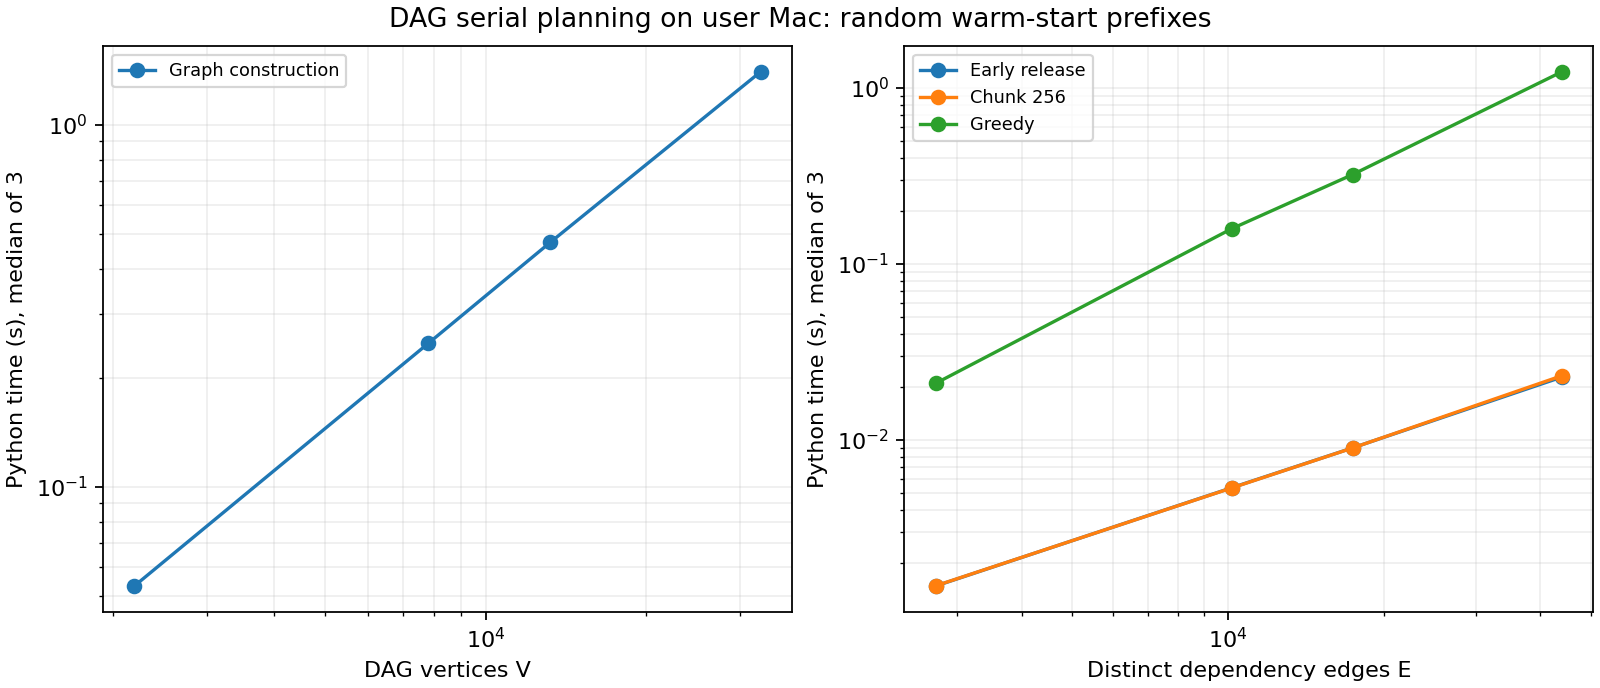
\includegraphics[width=0.96\linewidth]{figures/dag_runtime.png}
\caption{双对数坐标下，建图时间随顶点数、调度时间随边数变化。Mac 与 Vanda 时间不混成同一曲线。}
\label{fig:dag-runtime}
\end{figure}

\subsubsection{峰值内存与批量大小}
等大小 float32 面板模型将峰值存活数 $L$ 换算为 $4LN\lceil T/p\rceil$ 字节；这里 $T=1461$、$N=5876$、$p=1$。不计 halo、内存池保留缓冲、标签排名、算子及通信/PCA 工作区，因此不是 RSS。执行组数表示调度粒度，不是实测 MPI 同步或消息次数。

\begin{table}[htbp]
\centering\small
\begin{tabular}{lrrr}
\toprule
调度，29,955 条表达式 & 峰值面板 & 面板 GiB & 执行组（代理） \\
\midrule
保留根 & 32,290 & 1,032.67 & 3 \\
逐层早释放 & 17,730 & 567.02 & 3 \\
分块 1,024 & 4,850 & 155.11 & 33 \\
分块 256 & 4,086 & 130.67 & 129 \\
分块 64 & 3,896 & 124.60 & 512 \\
贪心 & 1,553 & 49.67 & 32,693 \\
\bottomrule
\end{tabular}
\caption{随机热启动批量的逻辑面板峰值。}
\label{tab:dag-memory}
\end{table}
早释放相对保留根降低峰值 45.1\%，分块 256 再降低 77.0\%。块大小从 256 降到 64 只再省 4.65\% 面板，执行组却接近四倍。贪心面板最少，并允许按需加载字段，但细粒度执行可能降低并行度。这体现内存与粒度的取舍，不能证明贪心运行最快。

\begin{figure}[htbp]
\centering
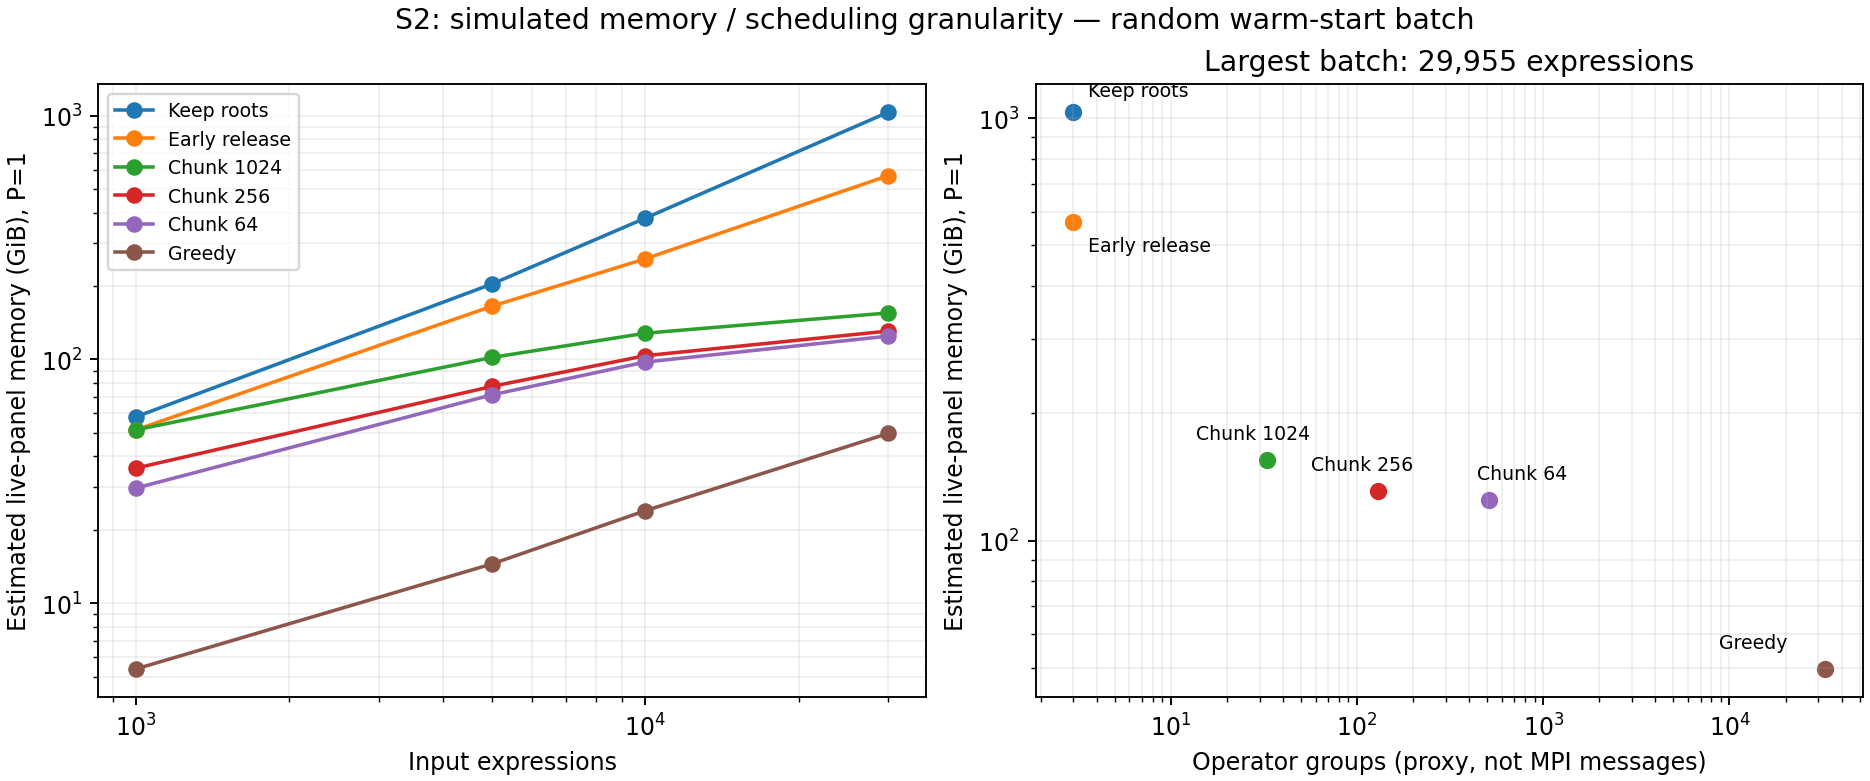
\includegraphics[width=\linewidth]{figures/dag_memory.png}
\caption{双对数坐标的模拟内存随批量变化（左），及最大批量的执行组数取舍（右）。执行组不是 MPI 消息数。}
\label{fig:dag-memory}
\end{figure}

\paragraph{小规模引擎检查（S4）。}
在 Vanda CPU 节点 CN-016，用交接的串行 C++ 导出驱动处理相同的前 200 条表达式，数据为 120 天 $\times$ 300 只股票。OpenMP、MPI、CUDA 均关闭（GCC 14.3.0，Release）。公式子批大小按 16、64、200 的顺序各跑三次，用 GNU time 计时。每个公式子批单独构图，不等同于同一张共享 DAG 的层内分块。

\begin{table}[htbp]
\centering
\begin{tabular}{rrrr}
\toprule
公式子批 & 墙钟中位数（s） & 范围（s） & RSS 中位数（MiB） \\
\midrule
16 & 1.60 & 1.53--1.93 & 25.42 \\
64 & 1.39 & 1.23--1.58 & 25.42 \\
200 & 1.29 & 1.26--1.75 & 34.53 \\
\bottomrule
\end{tabular}
\caption{实际单节点公式分块实验，每种配置运行三个独立进程。}
\label{tab:dag-s4}
\end{table}
九次运行均正常退出。服务器端逐条比较每次的 200 条评分与子批 200 的基准，只排除 chunk/slot 元数据，RankIC、fitness 和分段统计一致。已核对保留的验证记录和日志；审阅压缩包未包含原始评分文件。子批 64 比子批 200 的 RSS 中位数低 26.4\%。各配置 CPU 用户时间均约 0.88\,s，墙钟范围重叠，且未控制文件系统缓存和固定顺序，因此不判断运行速度优劣。驱动虽然关闭 $R$ 导出，仍计算签名行预处理。这只是公式划分的实际内存趋势验证，不是 S2 调度的精确验证。

\paragraph{对引擎实验的影响。}这些结果决定了后面实验中引擎如何计算一个批次。共享（表~\ref{tab:dag-sharing}）说明应先把整批表达式合并成一个 DAG 再计算：第~\ref{sec:experiments}~节的真实批次 10{,}000 条表达式合并后只有 12{,}083 个节点。根节点提前释放之后，峰值由最宽的一层决定（表~\ref{tab:dag-memory}），所以引擎还把宽层分块处理（第~\ref{sec:threads}~节）：该批次最宽一层有 8614 个节点，下面的实验单节点每块 1000 个节点，多节点每块 2000 个节点。分块不改变任何分数（表~\ref{tab:dag-s4} 与第~\ref{sec:threads}~节）。代价是 halo 交换从每层一次变为每块一次；我们没有比较分块与不分块的运行时间。

\subsection{因子计算与评估}

\subsubsection{串行运行时间与问题规模}
\label{sec:x1}
1 个进程、1 个线程。每次只改变一个维度：天数 $T$（真实数据的前缀）、股票数 $N$（前 $N$ 只股票）和批量大小（批次的前 $E$ 条表达式）。合成数据把 $T$ 和 $N$ 扩展到真实数据之外；这里用前 500 条表达式，因为天数放大 8 倍时表达式再多就放不进一个节点的内存（图~\ref{fig:x1}）。

\begin{table}[H]
\centering
\begin{tabular}{lrrr}
\toprule
维度 & 范围 & 总时间（s） & 斜率 \\
\midrule
$T$，真实，10{,}000 条 & 91 -- 1461 & 245 -- 5059 & 1.09 \\
$N$，真实，10{,}000 条 & 367 -- 5876 & 376 -- 5059 & 0.95 \\
$T$，合成，500 条 & 1461 -- 11688 & 540 -- 4825 & 1.05 \\
$N$，合成，500 条 & 5876 -- 23504 & 540 -- 2304 & 1.05 \\
批量大小，真实 & 625 -- 10{,}000 & 568 -- 5059 & 0.89 \\
\bottomrule
\end{tabular}
\caption{串行运行时间。斜率是在双对数坐标上对不含读数据的时间拟合得到的。}
\label{tab:x1}
\end{table}

整个批次单核需要 5059\,s（1.4 小时），这正是 Python 挖掘器每一代都很慢的原因。运行时间在每个维度上都接近线性，与第~\ref{sec:cost}~节的预测一致：算子每个节点是 $O(TN)$，RankIC 是 $O(TN\log N)$，所以合成数据上的斜率略大于 1。真实数据上 $T$ 的斜率（1.09）更大，是因为市场在扩张：短前缀覆盖的早期年份每天上市的股票更少。批量大小的斜率小于 1（0.89），因为批量越大，共享的子表达式越多：625 条表达式平均每条需要 2.1 个 DAG 节点，10{,}000 条只需要 1.2 个。RankIC 占串行时间的 70\%（3522\,s，算子 1536\,s），因为这个批次 83\% 的节点是根节点，每个根节点的 RankIC 都要对每天的横截面排序。

\begin{figure}[H]
\centering
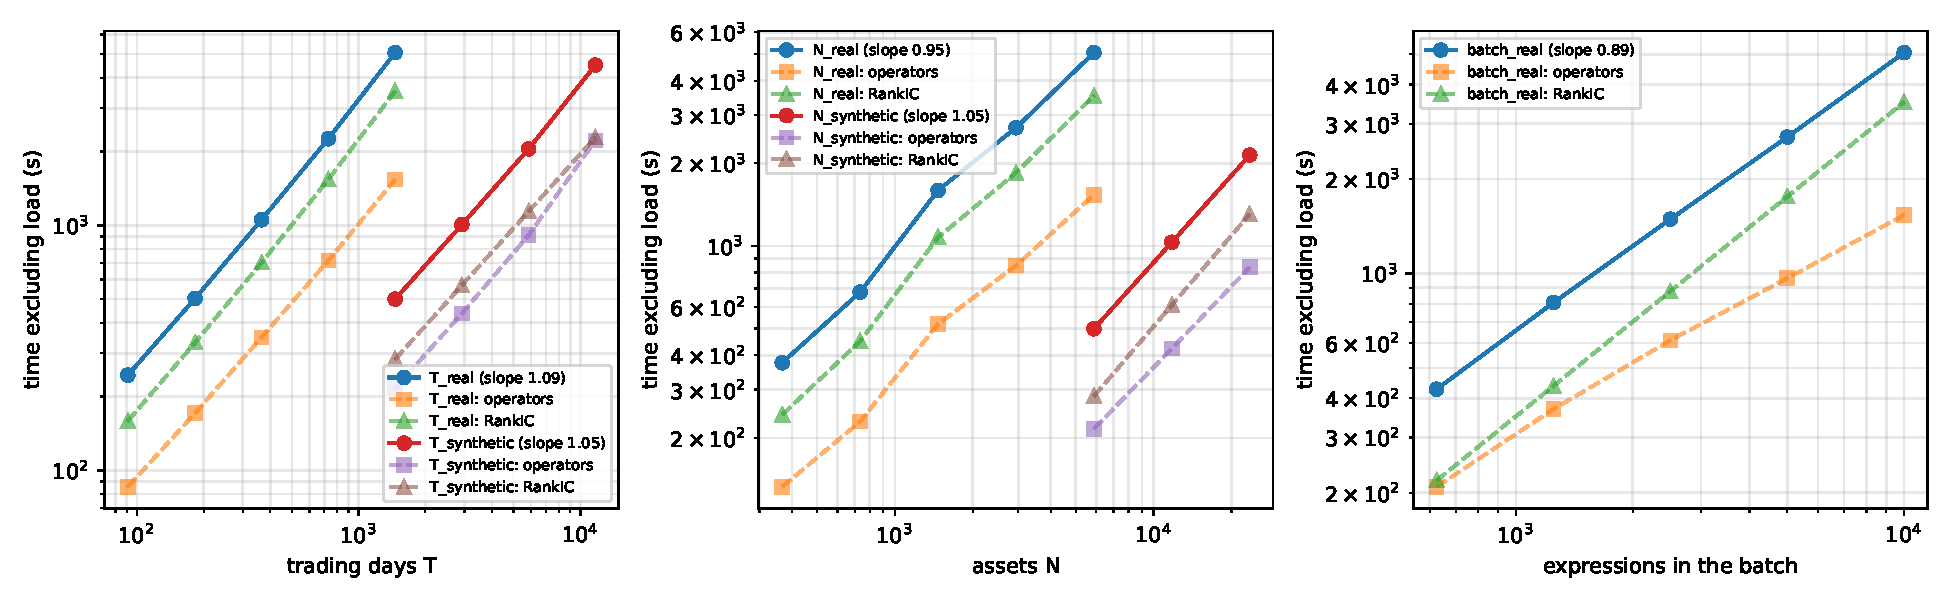
\includegraphics[width=\linewidth]{figures/x1_serial.pdf}
\caption{串行运行时间与 $T$、$N$、批量大小的关系，以及算子和 RankIC 两部分。真实数据：10{,}000 条表达式的批次或其前缀；合成数据：前 500 条表达式。}
\label{fig:x1}
\end{figure}

\subsubsection{强扩展（纯 MPI）}
每个进程 1 个线程，$H_0=0$；单节点 1 到 72 个进程，2 个和 4 个节点上分别是 144 和 288 个进程（表~\ref{tab:x2}，图~\ref{fig:x2}）。

\begin{table}[H]
\centering
\small
\begin{tabular}{lrrrrrrrrr}
\toprule
进程数 & 1 & 2 & 4 & 8 & 16 & 36 & 72 & 144 & 288 \\
节点数 & 1 & 1 & 1 & 1 & 1 & 1 & 1 & 2 & 4 \\
\midrule
时间（s） & 5060 & 2825 & 1534 & 815.7 & 436.4 & 241.3 & 142.7 & 94.1 & 75.0 \\
加速比 & 1 & 1.79 & 3.30 & 6.20 & 11.6 & 21.0 & 35.5 & 53.8 & 67.5 \\
效率 & 1 & 0.90 & 0.82 & 0.78 & 0.72 & 0.58 & 0.49 & 0.37 & 0.23 \\
\bottomrule
\end{tabular}
\caption{强扩展，10{,}000 条表达式，真实数据。}
\label{tab:x2}
\end{table}

各阶段的扩展情况差别很大。RankIC 完全是本地计算，从 3519\,s 降到 288 个进程时的 18.5\,s（190 倍）。算子从 1539\,s 降到 72 个进程时的 66\,s，但 288 个进程时也只降到 52\,s；halo 阶段从 16 个进程开始一直在 22--24\,s。288 个进程时每个日期块只有约 5 天，而交换节点最多需要 89 天的历史：每个进程要接收 1.7\,GB 的 halo 行，比它自己那一份面板还多，滚动窗口还要在每个块边界重新开始，所以每个进程的算子工作量不再随 $p$ 减少。等待在每个进程数下都很大（2 个进程时 2825\,s 中有 451\,s），这与第~\ref{sec:cost}~节说的日期块工作量不均一致：后半段时期上市股票更多。Karp--Flatt 串行比例从 2 个进程时的 0.12 降到 288 个进程时的 0.011，并且没有回升，所以损失不是一个不断增长的串行部分，而是不随 $p$ 减少的每进程开销：halo、块边界重启和负载不均。逐进程计时来区分这几项留作以后的工作。

\begin{figure}[H]
\centering
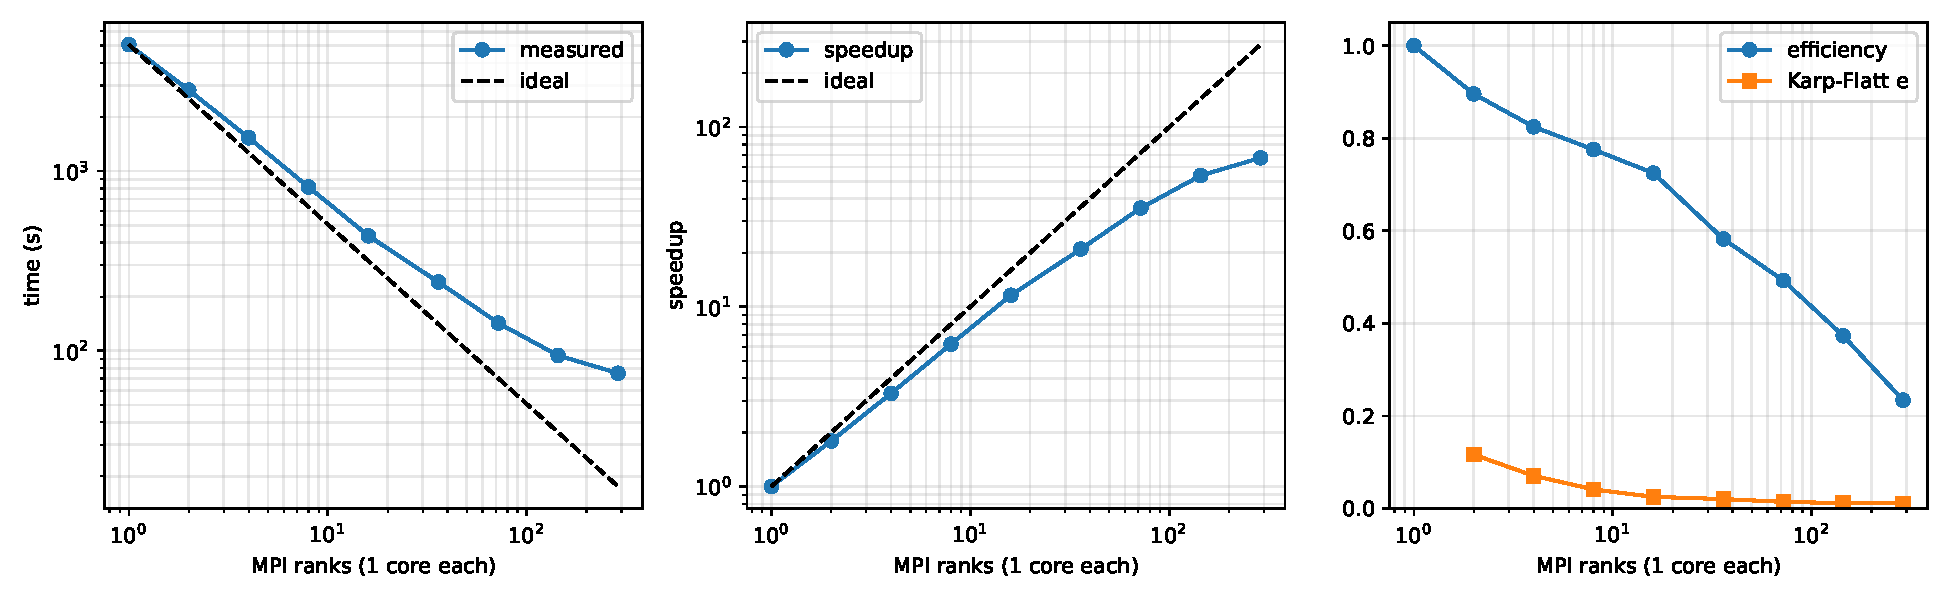
\includegraphics[width=\linewidth]{figures/x2_strong.pdf}
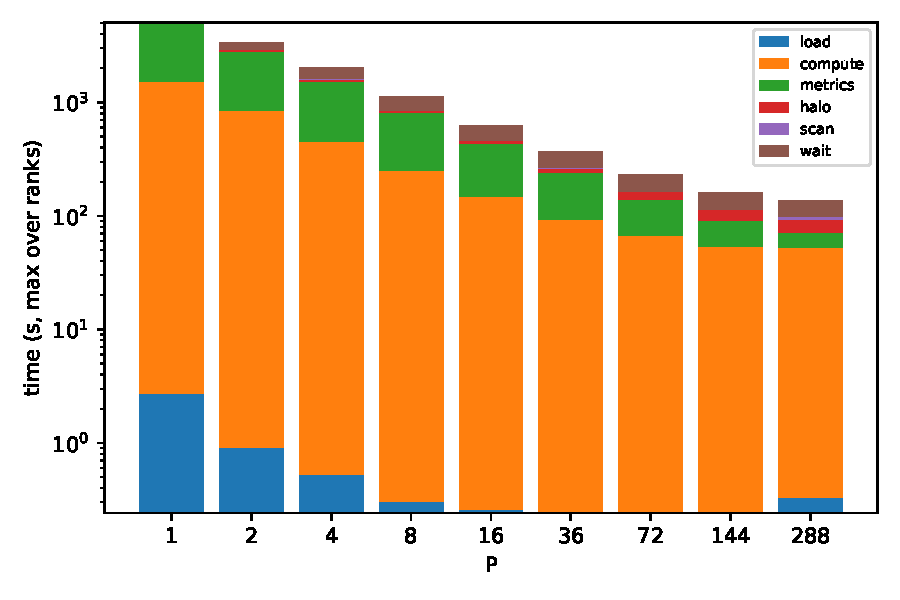
\includegraphics[width=0.6\linewidth]{figures/x2_strong_breakdown.pdf}
\caption{强扩展：时间、加速比、效率和 Karp--Flatt 指标（上）；各阶段时间（下）。}
\label{fig:x2}
\end{figure}

\subsubsection{弱扩展（纯 MPI）}
合成数据，每个进程 64 天（从 1 个进程的 $T=64$ 到 288 个进程的 $T=18432$），$N=5876$，用批次的前 1000 条表达式（1956 个 DAG 节点）；如果用整个批次，单节点 72 个进程每个 64 天会超出内存。

\begin{table}[H]
\centering
\begin{tabular}{lrrrrrr}
\toprule
进程数 & 1 & 2--16 & 36 & 72 & 144 & 288 \\
\midrule
时间（s） & 40.4 & $\approx$54.0 & 61.7 & 61.9 & 62.1 & 63.7 \\
效率 & 1 & 0.75 & 0.66 & 0.65 & 0.65 & 0.63 \\
\bottomrule
\end{tabular}
\caption{合成数据上的弱扩展，1000 条表达式。}
\label{tab:x3}
\end{table}

从 1 个进程到 2 个进程的下降来自 halo 交换（约 8.5\,s，36 个进程起也只升到 9.9\,s）以及相应的块边界计算。效率在 16 到 36 个进程之间再次下降，此时一个节点被占满，内存带宽被共享；之后在 2 个和 4 个节点上都保持在 0.63--0.65，说明跨网络带来的额外开销很小（表~\ref{tab:x3}，图~\ref{fig:x3}）。这里用合成数据，是因为真实数据无法随进程数增长；而且合成数据的日期块工作量相同，可以把通信和负载不均分开。

\begin{figure}[H]
\centering
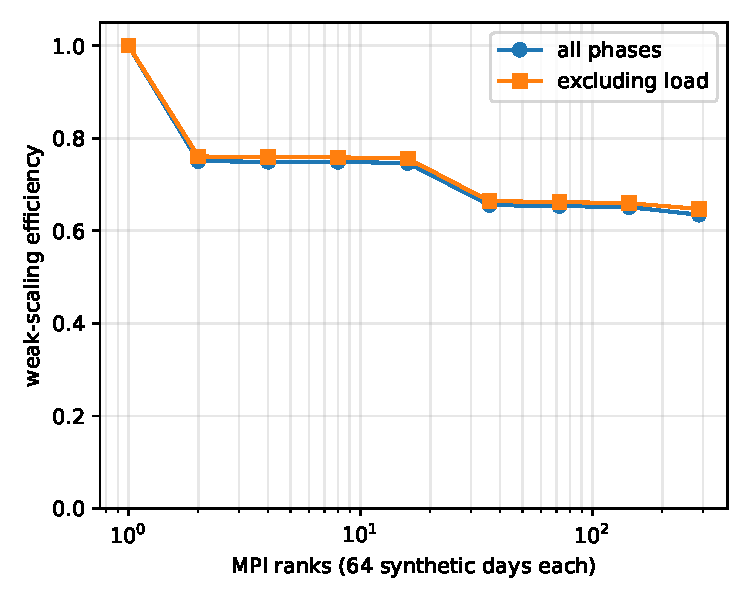
\includegraphics[width=0.45\linewidth]{figures/x3_weak.pdf}
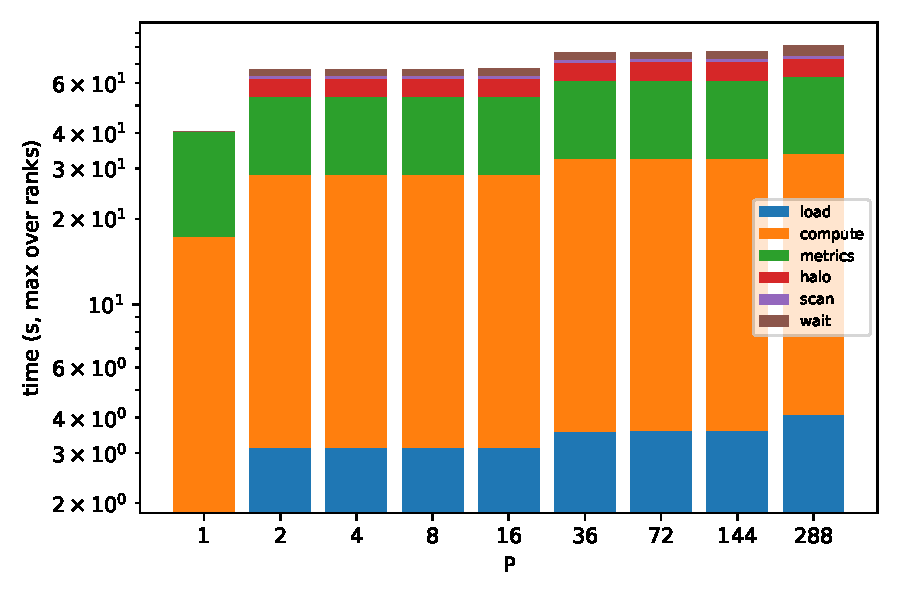
\includegraphics[width=0.5\linewidth]{figures/x3_weak_breakdown.pdf}
\caption{弱扩展效率和各阶段时间。}
\label{fig:x3}
\end{figure}

\subsubsection{通信}
\paragraph{halo 交换与冗余计算。}提高 $H_0$ 会用重算代替交换。纯 MPI 时，$H_0=10$ 几乎没有变化（交换节点从 1811 个变成 1591 个）；$H_0=30$ 时剩 715 个；$H_0\ge60$ 时只剩 53 个节点，每个进程的 halo 从 1.5--1.7\,GB 降到 40--45\,MB，代价是每个进程多算 60{,}944 行。但总时间反而增加：72 个进程从 142.7\,s 增到 159.1\,s（$+11\%$），144 个进程从 94.2\,s 增到 109.7\,s（$+16\%$），288 个进程从 72.0\,s 增到 86.7\,s（$+20\%$）（图~\ref{fig:x4} 左）。少发了 97\% 的数据，halo 时间却也增加了（72 个进程时从 23.7\,s 增到 31.1\,s），说明 halo 时间不是传输时间，而是等待左邻居算完这一层的时间，冗余计算让这段等待更长。对这个批次，全部交换（$H_0=0$）最好；混合划分的结论相同（72 个进程 $\times$ 4 个线程：$H_0=0$ 时 50.8\,s，$H_0\ge60$ 时 54\,s）。每个节点进程少时，$H_0$ 几乎没有影响：16 $\times$ 18 一直在 43.0--43.9\,s（$H_0=0$ 时 43.1\,s）；4 $\times$ 72 在 48.2 到 52.4\,s 之间波动（$H_0=0$ 时 55.0\,s），和 $H_0$ 没有单调关系。每个节点只有一个进程时，只有三对进程需要交换，能省下的本来就不多。

\paragraph{共享内存与网络。}同样数量的进程，尽量挤在少数节点上或分散到 4 个节点上：36 个进程在 1 个节点上 241.3\,s，分到 4 个节点 212.3\,s；72 个进程分别是 142.7\,s 和 126.4\,s；144 个进程在 2 个节点上 94.1\,s，在 4 个节点上 94.0\,s（图~\ref{fig:x4} 右）。分散更快：多出来的网络传输，代价比更多进程共享一个节点的内存带宽要小。

\paragraph{哪部分通信最多。}halo 远远占主导：每个进程每批发送 1.5--1.7\,GB，288 个进程合计约 500\,GB，而 4 个进程只有 6\,GB。ema 链需要 $p-1$ 次串行传递，每次每只股票两个数；连同它造成的等待，72 个进程时 0.83\,s，288 个进程时 4.8\,s。适应度只需要对 IC 汇总量做一次 \code{MPI\_Allreduce}，288 个进程时也不到 8\,ms。

\begin{figure}[H]
\centering
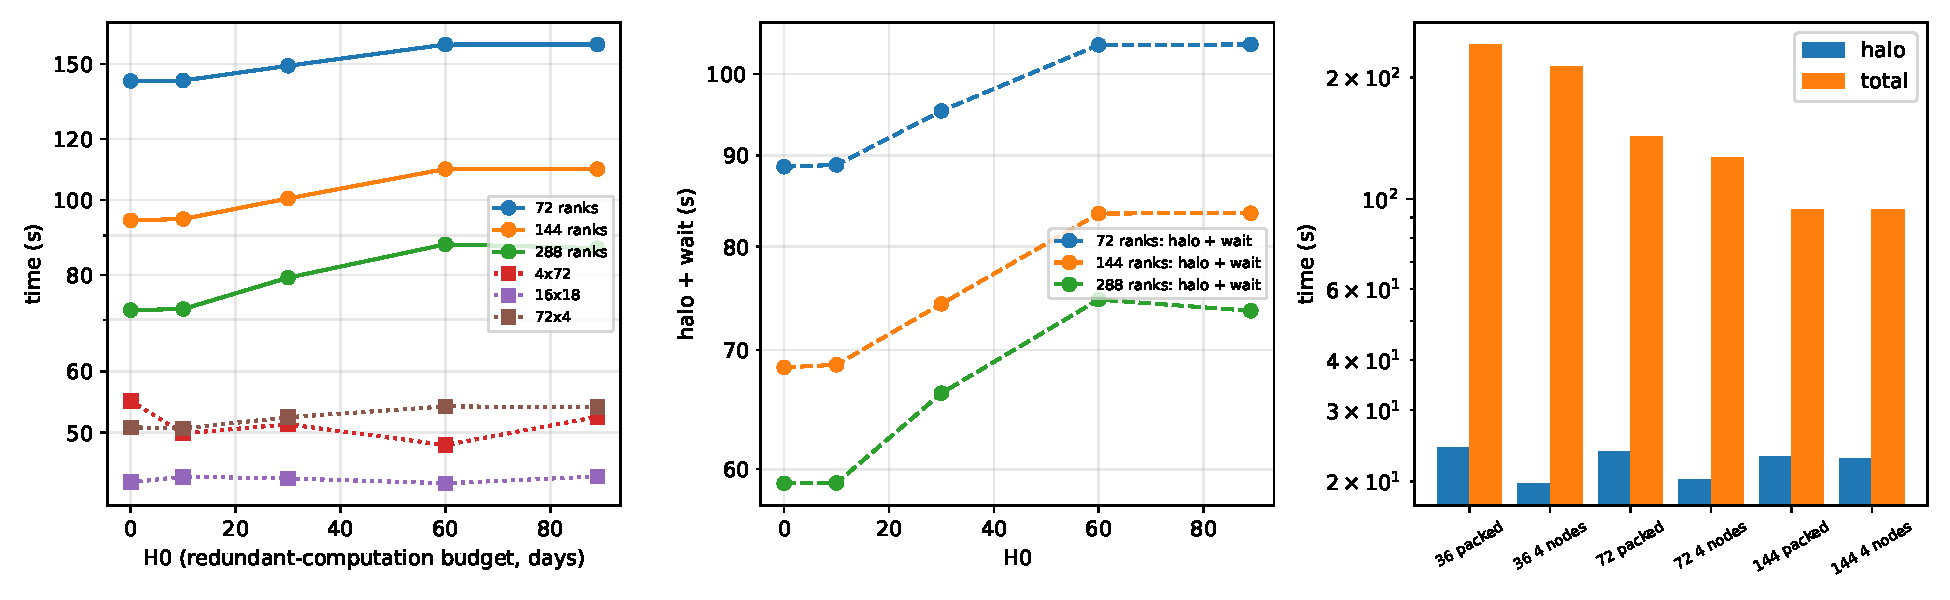
\includegraphics[width=\linewidth]{figures/x4_comm.pdf}
\caption{左：纯 MPI（实线）和混合划分（虚线）的总时间与 $H_0$ 的关系。中：halo 加等待时间。右：同样的进程数挤在少数节点上与分散到 4 个节点上。}
\label{fig:x4}
\end{figure}

\subsubsection{MPI + OpenMP}
\paragraph{单个进程。}1 个进程、2 到 72 个线程时，按算子并行分别是 2613、1349、690.9、360.9、200.2 和 110.3\,s，按节点并行分别是 2528、1267、635.9、321.9、166.6 和 89.2\,s（图~\ref{fig:x5} 左）。按节点并行在每个线程数下都更快，72 个线程时加速比 56.7（按算子 45.9）。两个算子层分别有 3337 和 8614 个节点，每个线程总有活干，也不需要为每个算子开一次并行区域。在一个节点上，72 个线程（89.2\,s）比 72 个进程（142.7\,s）快 1.6 倍，因为不需要 halo 交换，也没有块边界重启。

\paragraph{288 个核。}把 4 个节点划分为进程数 $\times$ 线程数（表~\ref{tab:x5}，图~\ref{fig:x5} 右）。

\begin{table}[H]
\centering
\begin{tabular}{lrrrrrrr}
\toprule
进程 $\times$ 线程 & 288$\times$1 & 144$\times$2 & 72$\times$4 & 36$\times$8 & 16$\times$18 & 8$\times$36 & 4$\times$72 \\
\midrule
按算子（s） & 75.0 & 61.4 & 50.8 & 47.5 & 43.1 & 43.6 & 55.0 \\
按节点（s） & 75.0 & 48.9 & 37.7 & 32.8 & 29.3 & 28.1 & \textbf{27.8} \\
\bottomrule
\end{tabular}
\caption{288 个核划分为 MPI 进程和 OpenMP 线程，10{,}000 条表达式。}
\label{tab:x5}
\end{table}

按节点并行时，用线程替换进程，时间一路下降；最好的是 4 个进程 $\times$ 72 个线程（每个节点一个进程）：27.8\,s，比同样 288 核的纯 MPI 快 2.7 倍，比单核快 182 倍；8 $\times$ 36（28.1\,s）和 16 $\times$ 18（29.3\,s）也几乎一样快。每个进程仍要接收约 1.5\,GB 的 halo，所以 halo 总流量和进程数成正比，halo 阶段从 288 个进程时的 22\,s 降到 4 个进程时的 1.5\,s。按算子并行在每种划分下都更慢，差距主要在评估上：按算子并行时，RankIC 在每种划分下都约 29\,s，按节点并行约 18\,s。每个进程 72 个线程时，按算子并行又变慢（55.0\,s）：每个算子都要在两个 socket 的 72 个核上开一次并行区域。

\begin{figure}[H]
\centering
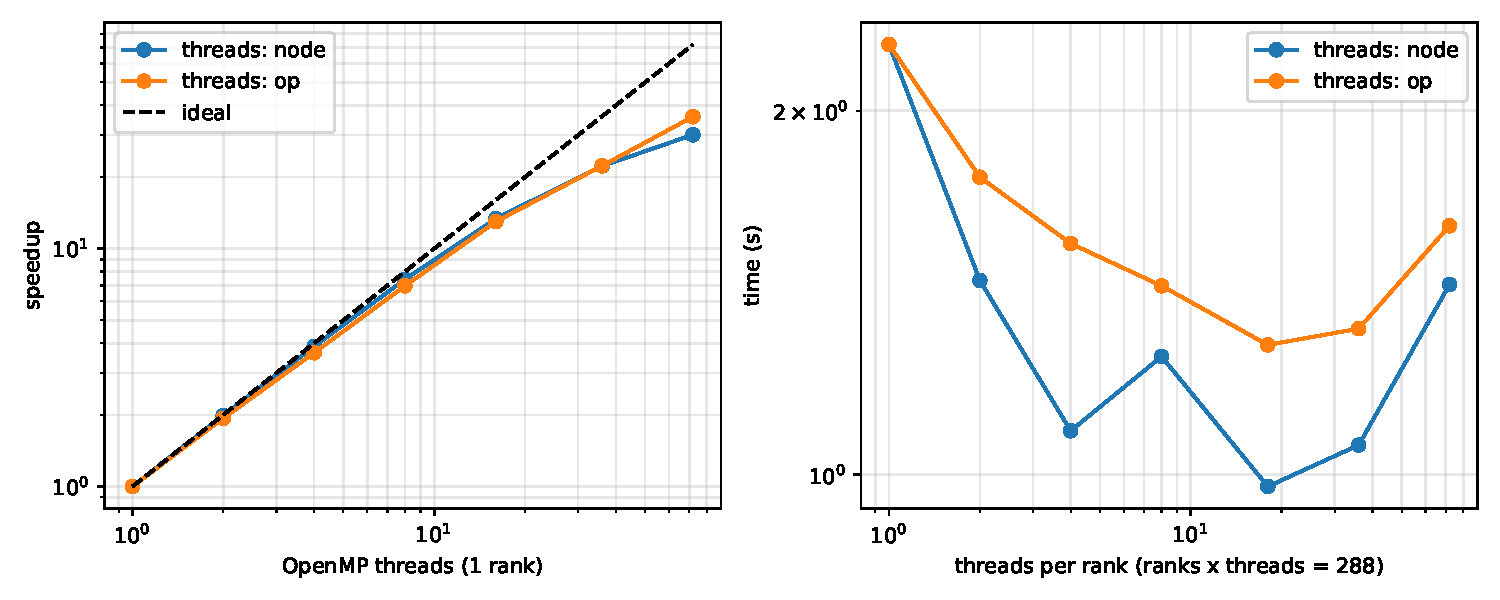
\includegraphics[width=\linewidth]{figures/x5_hybrid.pdf}
\caption{左：单个进程使用 OpenMP 线程的加速比。右：288 个核划分为进程 $\times$ 线程，两种线程策略。}
\label{fig:x5}
\end{figure}

\subsubsection{大规模一致性}
\label{sec:v}
分布式结果和串行结果按第~\ref{sec:validation}~节的标准比较（候选的有效性相同，且 $|\Delta\text{适应度}|\le10^{-5}$）。这项检查要保留所有根节点的结果，还要在 0 号进程上再跑一遍串行引擎，所以只用批次的前 1000 条表达式。72 个进程（单节点）、288 个进程（4 个节点）、16 个进程 $\times$ 18 个线程按节点并行（4 个节点）都通过，全部开启了分块；16 个进程（每块 300 个节点）和 4 个进程 $\times$ 4 个线程（每块 250 个节点）也通过。

\subsection{PCA 签名与相似度}

\subsubsection{串行代价}
\label{sec:pca-results}
本节的 PCA 输入单独构造：深度 3 随机提案导出 9388 个非恒定矩阵 $R$，其中 8866 个候选可用于 QD，四步幂迭代得到 2988 个档案成员。下层基因池由随机提案组成；它与前述深度 2 的固定 10{,}000 条表达式引擎批次是不同输入。下面先考察 128 个真实面板上的规模变化，再报告整批 $R$ 的性能。

真实规模实验先由原引擎计算 128 个因子面板，再固定面板值，改变抽样间隔（1、2、5、10、20）、股票前缀（367、734、1469、2938、5876）、批量 $B$ 和步数 $k$，共 19 个配置。每组预热一次、计时三次，并重新排名、求签名和执行 QD。八线程生成因子耗时 86.410\,s，单列；PCA 使用单线程，包含抽样复制、排名、求解和准入，序列化另计。

\begin{figure}[H]
\centering
\includegraphics[width=0.82\linewidth]{\PCAFigureDir/real_problem_size.png}
\caption{128 个真实面板上的 PCA 规模实验。固定面板值后改变 $B$、抽样天数 $m$、股票数 $N$ 和步数 $k$。}
\label{fig:pca-real-size}
\end{figure}
图~\ref{fig:pca-real-size} 中，耗时随批量、抽样天数和股票数增长；步数主要影响求解部分，排名和准备仍占较大比例。矩阵向量乘的主要工作量约为 $O(BmNk)$，合成维度实验也显示 $B,m,N$ 方向近似线性增长。股票前缀实验没有在较小股票池重新计算截面算子或 RankIC，因此反映的是 PCA 输入规模变化，而非重新挖掘一个较小股票池的成本。

\subsubsection{GPU kernel 与 CPU 对比}
表~\ref{tab:pca-kernels} 分别测量排名、迭代乘法和相似度。FP32/FP64 指迭代精度；排名及相似度粗算均为 FP32。排名时间明显高于两类乘法。改用 FP64 后迭代乘法接近翻倍，但排名不变，因此整个流程不会按相同比例变慢。
\begin{table}[H]
\centering\small
\caption{GPU 分项计时，单位 ms；每组预热一次，三次测量取中位数。}
\label{tab:pca-kernels}
\begin{tabular}{lrrrr}
\toprule
迭代精度 & 批量 $B$ & 排名 & 矩阵向量乘 & 相似度 \\
\midrule
FP32 & 8  & 21.212  & 0.964  & 0.097 \\
FP32 & 32 & 84.694  & 3.737  & 0.156 \\
FP32 & 64 & 169.285 & 7.450  & 0.273 \\
FP64 & 8  & 21.209  & 1.773  & 0.098 \\
FP64 & 32 & 84.694  & 7.023  & 0.157 \\
FP64 & 64 & 169.289 & 14.017 & 0.272 \\
\bottomrule
\end{tabular}
\end{table}

处理全部 9388 个已构造的 $R$ 时，72 核 CPU 的 \code{date} 布局用时 13.366\,s，单张 A40 为 64.766\,s，同节点双 A40 为 36.713\,s（图~\ref{fig:pca-total}）。该范围包含读取、准备、传输、计算、相似度、准入和循环内签名写入，不含因子生成；MPI 启动、GPU 初始化及最终 JSON 序列化另计，写入未包含 fsync 持久化保证。输入已完成排名，这组总时间不包含 GPU 排序。CPU 使用 72 个进程、FP64、批量 576；GPU 使用 1/2 个进程、FP32、批量 128。因此它比较的是这些实际资源和实现配置，而非仅改变设备的一项受控实验。
\begin{figure}[H]
\centering
\includegraphics[width=0.54\linewidth]{\PCAFigureDir/cpu_gpu_end_to_end.png}
\caption{同一批 9388 个 $R$ 的 PCA 流程时间。CPU 与 GPU 使用各自所列资源配置。}
\label{fig:pca-total}
\end{figure}

表~\ref{tab:pca-total-stages} 显示，CPU 的读取由 72 个进程分担，而 GPU 路径只有 1/2 个主机进程。单卡纯 GEMV 内核中位数为 1.090\,s，远小于整批墙钟；读取、主机数据准备、上传和同步需要一起优化。\code{solve} 阶段包含 GPU 准备及计算，其内部计时有嵌套。由此可见，当前配置的总时间较慢，不能推出 GPU 乘法本身较慢。

\begin{table}[H]
\centering\small
\caption{整批已排名 $R$ 的配置及阶段时间中位数，单位 s。求解阶段包含准备及嵌套子阶段，不能与 GPU 内核或通信计时直接相加。}
\label{tab:pca-total-stages}
\begin{tabular}{lrlrrrr}
\toprule
配置 & MPI 进程 & 求解精度 & 批量 $B$ & 读取 & 求解阶段 & 总时间 \\
\midrule
CPU & 72 & FP64 & 576 & 1.496 & 11.537 & 13.366 \\
单 A40 & 1 & FP32 & 128 & 34.170 & 27.429 & 64.766 \\
双 A40 & 2 & FP32 & 128 & 18.845 & 17.479 & 36.713 \\
\bottomrule
\end{tabular}
\end{table}


顺序准入计时包含 FP64 复核和档案状态维护，排除相似度预计算。按每次运行的 $T_{\rm adm}/T_{\rm total}$ 计算，再对三次运行取中位数，72 核 CPU、单 A40、双 A40 的占比分别为 8.12\%、1.48\%、2.64\%。这些比例对应本节 PCA 流程；整个 GP 的串行比例需按完整循环计时。

独立 cuBLAS 参照使用相同显存输入，严格 FP32、关闭 TF32（\href{https://docs.nvidia.com/cuda/archive/12.9.1/cublas/index.html}{cuBLAS 文档}）。每块执行 50 次，三个块取中位数，排除预热、传输、分配和归一化。手写版本融合了绝对值，因此表~\ref{tab:cublas} 以库 GEMM 加 abs 的时间作对应比较，纯 GEMM 另列。其中 abs 表示逐元素取绝对值。表中的加速比为手写耗时除以库 GEMM+abs 耗时，大于 1 表示库实现更快。库实现快 1.45--3.89 倍，说明手写乘法仍有优化空间；这一差距不能直接换算成整个 GP 的加速比。cuBLAS 只用于参照，生产目标仍使用手写实现。
\begin{table}[H]
\centering\small
\caption{相似度操作与 cuBLAS 的独立对照，时间单位为 $\mu$s。}
\label{tab:cublas}
\begin{tabular}{rrrrrr}
\toprule
$B$ & 档案数 $A$ & 手写相似度 & 库 GEMM & 库 GEMM+abs & 库加速比 \\
\midrule
128 & 50000 & 1465.10 & 282.17 & 376.59 & 3.89 \\
32  & 16384 & 121.53  & 47.66  & 51.45  & 2.36 \\
64  & 16384 & 230.63  & 53.35  & 62.32  & 3.70 \\
8   & 16384 & 66.31   & 43.72  & 45.81  & 1.45 \\
\bottomrule
\end{tabular}
\end{table}

\subsubsection{MPI + CUDA 扩展性}
CPU 三种布局的强扩展见图~\ref{fig:pca-scaling}。低进程数时增加进程能减少时间，随后收益趋缓，部分配置回升。\code{date} 每轮的向量归约不随进程数缩短，\code{transpose} 承担重分布，\code{factor} 依赖并行读取。弱扩展中，保持每进程完整矩阵等价工作量后，时间仍增长且有波动，效率未稳定在 1 附近。个别超线性点应结合节点和运行条件解释。
\begin{figure}[H]
\centering
\includegraphics[width=\linewidth]{\PCAFigureDir/strong_scaling.png}
\medskip
\includegraphics[width=0.75\linewidth]{\PCAFigureDir/weak_scaling.png}
\caption{PCA 模块的 CPU 强扩展（上）与弱扩展（下）。三种布局的读取、准备和通信范围不同，比较以各自总时间为准。}
\label{fig:pca-scaling}
\end{figure}

同节点双 A40 相对单卡加速 1.764 倍，日期块分给两张卡，范数与右向量通过显存 Allreduce 合并。两节点各一卡另有正确性检查，不能用同节点性能代替跨节点加速比。档案规模实验固定 128 个候选；在所测大档案配置中，签名分片降低了处理时间，但每个候选仍需 MAXLOC 和顺序决定，通信限制了扩展收益。

\subsubsection{签名与准入判定的一致性}
整批 FP32/FP64 对照中，动作变化数、动作/最近 key/替换 key 三元组变化数、最终成员对称差均为 0。提供签名重放与从相同 FP32 $R$ 重算的结果也保持一致。这支持本批输入下的实现及精度选择；算法、步数和初值的变化则在下一节单独比较。

\paragraph{后端与档案状态检查。}
给定相同签名，逐候选核对动作、最近 key、替换 key 和最终成员，CPU、CUDA、MPI 分片与原 Python 参考一致。边界覆盖 $0.90$ 附近、最大值并列、同 key、质量差恰为 $0.002$ 及无效签名。整批运行与分两批读取快照的最终档案状态一致；实际 GP 还检查了中断恢复和后端身份。方向误差与准入阈值对应不同的量，是否改变档案应以上述逐项决定核对为准。

\paragraph{实际 GP 衔接与 16 核校准。}
接口验证先在 120 天、300 只股票、6 个字段上完成三个深度各一代的运行。CPU/MPI 和 CUDA 均保留 24 个档案成员，GP 墙钟分别为 189.463\,s 和 268.381\,s。随后使用全部 1461 天、5876 只股票和 132 个字段，设置种群 64、热启动倍数 3、基因池上限 32，深度 1、2、3 各一代；窗口为 1/5/10/15/20/30/60，每五天抽样，四步 FP64 幂迭代。表~\ref{tab:live-gp} 给出这套配置的运行结果。

\begin{table}[H]
\centering\small
\caption{全数据维度上的三层 GP 衔接实验。准备时间与 GP 墙钟分别计时；共享 CPU 行是后续单独运行。}
\label{tab:live-gp}
\begin{tabular}{lrrrrrr}
\toprule
后端 & MPI 进程 & 每进程线程 & 准备 / s & GP 墙钟 / s & 评价数 & 档案数 \\
\midrule
CPU & 16 & 1 & 371.334 & 233.940 & 1450 & 325 \\
CUDA（1 A40） & 1 & 16 & 0.046 & 336.705 & 1450 & 325 \\
CPU（共享） & 16 & 1 & 0.052 & 234.358 & 1450 & 325 \\
\bottomrule
\end{tabular}
\end{table}

CPU 使用 16 个单线程 MPI 进程；CUDA 使用一个进程、16 个 CPU 线程和一张 A40，实际预留 36 核、240 GB。两条路径的因子值和 RankIC 都由 CPU 计算，GPU 承担排名、PCA 和相似度。首次 CPU 运行完成字段分析；CUDA 与后续共享 CPU 运行复用了核对身份的字段缓存，所以准备时间不能当成算法速度对比。GP 墙钟包含 MPI 子进程启动、因子引擎、PCA、QD、Python 控制及检查点。

CPU/CUDA 两次运行的最终 325 个 key 相同，但数值不逐位相同：共同成员质量的最大绝对差为 $4.70977\times10^{-5}$，FP32 签名分量最大绝对差为 $0.00370505$。累计评价数包括热启动和各层搜索，因此不等于种群数乘以代数；档案跨批次积累，成员数也可超过单代种群。

后续共享资源校准在 CN-161（Xeon Platinum 8452Y）申请 16 核、112 GB，保留相同三层设置，得到 234.358\,s 和 325 个成员。另固定抽取 1000 个去重的实际表达式，以相同顺序完成因子、RankIC、PCA 和 QD；一次预热、三次测量的批次墙钟中位数为 64.648\,s，范围 64.308--65.301\,s。每次均与原 Python QD 核对决定和最终成员，同一布局的重复数值输出逐位一致。输入校验单列为 102.041\,s。

整个校准作业包含上述重复测试与三层 GP，共用时 10 分 28 秒。该机器由其他作业共享，因此这组时间用于验证资源路线和实际衔接，不与独占节点结果直接构造扩展加速比；它与第~\ref{sec:x1}~节的 10{,}000 条固定表达式也有不同输入和计时范围。

\subsection{幂迭代与 Lanczos}

\subsubsection{精度与迭代次数}
\label{sec:solver-results}
对完整 NumPy SVD 的第一左奇异向量 $u_{\mathrm{ref}}$，定义方向误差
\begin{equation}
 e=1-\frac{|s^\top u_{\mathrm{ref}}|}{\|s\|_2\,\|u_{\mathrm{ref}}\|_2}.
 \label{eq:direction-error}
\end{equation}
绝对值消除符号影响，严格目标取 $e\le10^{-6}$。误差越接近 0，表示计算方向越接近 SVD 参考方向。它与准入使用的 Pearson 相似度不是同一个量，因此不能直接与 $0.90$ 阈值比较。实验还以相对特征残差诊断 $RR^\top s$ 与其 Rayleigh 商对应方向的差异；残差另需两次矩阵向量乘。

9388 个矩阵中，13.9\% 的 $\sigma_2/\sigma_1>0.9$。seed=0 的四步幂迭代有 7053 个矩阵没有达到严格目标。图~\ref{fig:solver-convergence} 同时按步数和实际矩阵向量乘次数比较：随着预算增加，Lanczos 更快接近 SVD 参考。受控谱实验也显示，两个主方向越接近，幂迭代的收敛越慢。这里衡量有限步近似，而非程序是否出错。
\begin{figure}[H]
\centering
\includegraphics[width=0.92\linewidth]{\PCAFigureDir/convergence.png}
\caption{幂迭代与 Lanczos 的方向误差，分别按步数（左）和矩阵向量乘次数（右）比较。}
\label{fig:solver-convergence}
\end{figure}

\subsubsection{计算代价}
先用 SVD 离线确定各矩阵达到目标的迭代预算，上限为十步；两种方法均执行全部 9388 个矩阵，将未达标者单列，再在共同达标的 6679 个矩阵上比较成本（表~\ref{tab:solver-cost}、图~\ref{fig:solver-cost}）。“共同达标”指两种算法都在十步内达到同一误差阈值；只在这部分矩阵上比较时间，是为了避免把精度不同的运行直接比较。Lanczos 达标数更多，共同集合求解时间由 10.235\,s 降至 8.154\,s，减少约 20.3\%。
\begin{table}[H]
\centering\small
\caption{共同精度比较。达标/未达标统计针对全集；后三列仅针对共同达标的 6679 个矩阵。逻辑载荷按十进制 GB 换算。}
\label{tab:solver-cost}
\begin{tabular}{lrrrrr}
\toprule
算法 & 达标数 & 十步未达标 & 求解 / s & Allreduce 次数 & 逻辑载荷 / GB \\
\midrule
幂迭代 & 6679 & 2709 & 10.235 & 78747 & 1.694 \\
Lanczos & 8179 & 1209 & 8.154 & 109162 & 1.127 \\
\bottomrule
\end{tabular}
\end{table}
\begin{figure}[H]
\centering
\includegraphics[width=0.93\linewidth]{\PCAFigureDir/full_accuracy_cost.png}
\caption{共同达标集合的求解时间、归约次数与逻辑通信载荷。}
\label{fig:solver-cost}
\end{figure}

Lanczos 的重正交化增加了标量归约，但达到目标所需的迭代预算也不同，所以更多归约调用仍可能对应更少的总载荷。逻辑字节不等于实际网络流量。逻辑载荷按归约数组的字节数累计，实际网络传输还取决于 MPI 使用的通信算法。该实验预留 16 核、111 GB，实际使用 8 个单线程 MPI 进程；双方均逐因子归约，未采用生产幂迭代的批量归约。纯求解计时排除残差诊断、输入缓存和记录。这里是离线选定预算的成本比较，生产程序仍按固定步数运行。

\subsubsection{对准入判定的影响}
以 seed=0、四步幂迭代为基准，固定候选顺序和质量，只改变签名算法与步数。动作变化数统计加入、替换、拒绝这三类决定的变化；最近记录变化数还包含决定不变、但匹配对象改变的情况。表~\ref{tab:decision-change} 显示，八步幂迭代改变了 637 个动作，最终成员对称差为 372。对称差同时计入移入和移出，不等于替换次数。例如，一个成员移出、另一个成员移入，对称差记为 2。完整实验保存 60 条轨迹，多个起点也出现差异（图~\ref{fig:decision-change}）。
\begin{table}[H]
\centering\small
\caption{相对四步幂迭代基线的准入变化。}
\label{tab:decision-change}
\begin{tabular}{lrrrr}
\toprule
算法 & 步数 $k$ & 动作变化数 & 最近记录变化数 & 最终成员对称差 \\
\midrule
幂迭代 & 2 & 960 & 5984 & 568 \\
幂迭代 & 4 & 0 & 0 & 0 \\
幂迭代 & 8 & 637 & 4204 & 372 \\
Lanczos & 2 & 1373 & 6992 & 942 \\
Lanczos & 4 & 469 & 3702 & 233 \\
Lanczos & 8 & 758 & 4945 & 461 \\
\bottomrule
\end{tabular}
\end{table}
\begin{figure}[H]
\centering
\includegraphics[width=0.72\linewidth]{\PCAFigureDir/decision_sensitivity.png}
\caption{算法、预算和初始向量对准入动作的影响。}
\label{fig:decision-change}
\end{figure}

因此，同输入下复现原四步基线，与换用更精确的方向后保持名单不变，是两个不同目标。顺序档案会传播早期决定的差异，提高方向精度也不能单独证明因子质量得到改善。

%======================================================================
\section{讨论}

\subsection{各部分如何并行}
表~\ref{tab:parallel-summary} 汇总各模块的并行方式与通信。因子引擎按日期划分，截面计算保持本地，时序算子交换历史；PCA 延续日期划分，但每轮还需合并范数和右向量。GPU 能加速排名、乘法和相似度，顺序档案更新仍保留串行依赖。
\begin{table}[H]
\centering\small
\caption{各模块的并行方式、逻辑通信量与主要瓶颈。halo 按进程计，其余按批计。}
\label{tab:parallel-summary}
\resizebox{\linewidth}{!}{%
\begin{tabular}{p{2.2cm}p{2.7cm}p{4.1cm}p{4.1cm}}
\toprule
模块 & 并行方式 & 主要 MPI 通信量或方式 & 主要限制 \\
\midrule
因子算子 & MPI + OpenMP & halo 每进程每批约 1.5--1.7\,GB；ema 为 $p-1$ 次、每次 $2N$ 个数 & 回看历史、负载不均 \\
RankIC 与适应度 & 每日本地、全局汇总 & $O(E)$ 个评分统计量归约 & 排名与内存带宽 \\
抽样排名 & CPU / CUDA & 无跨进程排名交换 & 排序、数据传输 \\
PCA（date） & MPI + CPU/CUDA & 每轮 $B+BN$ 个数归约，最终再归约 $B$ 个数 & 归约量不随进程数缩小 \\
PCA（transpose） & Alltoallv + 本地求解 & $O(BmN)$ 数据重分布，$O(Bm)$ 签名汇集 & 准备、重分布、读取 \\
集中档案 & CPU/CUDA 粗算、CPU 复核 & $O(Bm)$ 签名汇集 & 顺序准入 \\
分片档案 & MPI 比较 + MAXLOC & 每候选一次 MAXLOC & 通信、元数据处理 \\
\bottomrule
\end{tabular}}
\end{table}

原引擎批次中，halo 的逻辑发送量最大：288 个进程合计约 500\,GB，而 IC 汇总归约只占很少时间。PCA 的限制不同，日期划分下每次右向量归约的数据量不会随进程数减小。实际 GP 另包含启动、快照准备、Python 控制和检查点，因此应按目标流程的墙钟选择配置，不能只比较单个内核。

\subsection{关于数据的结论}
真实数据中每日股票数从 2636 增至 4845，等长日期块并不等工作量，这是引擎等待与扩展损失的重要来源。固定尺寸 $R$ 的规模实验刻画的是 PCA 成本，不直接测量这种引擎负载变化。分布式归约和面板精度还可能影响近似相等的数值；因此数值一致性、准入一致性和完整进化结果分别核对。

表~\ref{tab:qd-quality} 与图~\ref{fig:qd-quality} 考察深度 3 随机提案，比较 8866 个有效候选与四步幂迭代形成的 2988 个档案成员。这里不是前述三层 GP 的 325 个成员，也不同于验证中引用的 1481 个历史已选因子。
\begin{table}[H]
\centering\small
\caption{随机提案与 QD 档案的样本内绝对平均 RankIC。}
\label{tab:qd-quality}
\begin{tabular}{lrrrrrr}
\toprule
集合 & 数量 & 最小值 & 25\% 分位 & 中位数 & 75\% 分位 & 最大值 \\
\midrule
有效候选 & 8866 & $1.82136\times10^{-7}$ & 0.0086576 & 0.0230372 & 0.0434855 & 0.107231 \\
QD 档案 & 2988 & $1.82136\times10^{-7}$ & 0.00349045 & 0.0107784 & 0.0240051 & 0.107231 \\
\bottomrule
\end{tabular}
\end{table}
\begin{figure}[H]
\centering
\includegraphics[width=0.68\linewidth]{\PCAFigureDir/rankic_distributions.png}
\caption{有效候选与 QD 档案的样本内 RankIC 分布。}
\label{fig:qd-quality}
\end{figure}

档案中位数低于原候选集合。QD 比较的是相似模式内部的质量，并非只保留 RankIC 最大的一部分：质量较低但模式不同的因子仍可加入。该分布说明了质量与多样性的取舍，不能单独作为投资收益或样本外表现的证据。

精度选择也影响排名：float64 数值转为 float32 后可能形成新的并列值。因此需区分面板存储导致的排名变化，与相同 FP32 $R$ 上求解实现的差异。前者用相同舍入后的输入核对 RankIC，后者核对签名和完整准入轨迹；本批 FP32/FP64 求解没有改变准入动作或最终成员，不能据此推断任意输入都保持一致。

\subsection{后续工作}
因子引擎可继续按实际工作量加权分配日期，减少股票池扩大造成的等待；用 \code{MPI\_Exscan} 组织 ema 的跨块传递，并融合逐元素算子，减少中间面板和内存往返。

GP 可进一步研究异步稳态进化，重叠 CPU 因子计算与 GPU PCA，提前准备随机移民，不必等当前一代的 PCA 完成后再生成；同时减少每批独立子进程和档案快照的成本。分块应根据显存预算选择；若只有 24\,GB 显存，可缩小批量、按需上传，避免同时保留过多根面板。算法方面，可研究基于残差的在线停止，但应同时测量诊断开销和准入变化，不能只以方向误差更小代替完整流程评价。

%======================================================================
\section{结论}
本文将原 Python GP 的批量评价迁移到 C++，以 DAG 共享减少重复计算，以日期划分组织 MPI + OpenMP 因子引擎，并接入手写 CPU/CUDA 的 PCA、相似度和顺序 QD。原引擎固定批次从单核约 5060\,s 降至 288 核纯 MPI 的 75.0\,s；同为 288 核时，按节点线程策略的 $4\times72$ 配置达到 27.8\,s。这些收益来自本地计算减少与共享内存复用，后期则受到 halo、边界重启和不均衡限制。

PCA 实验表明，排名、准备、通信和准入必须与乘法一起计时。双 A40 比单卡快 1.764 倍，但本批流程仍以 72 核 CPU 配置更快。Lanczos 在十步内达标的矩阵更多，并在共同精度集合上减少约 20.3\% 求解时间；同时，改变算法或预算会改变部分档案成员。全数据维度上的三层 GP 运行与共享 16 核校准进一步验证了因子引擎、PCA、QD、后续进化和检查点之间的衔接。

\section*{AI 工具的使用}
本文使用 ChatGPT 辅助讨论。
\clearpage

\appendix
\section{代码结构、编译与运行}
主要源码见项目的 \href{https://github.com/houjiacheng435-a11y/GP_factor_miner_distributed/tree/pca-implementation}{GitHub 仓库（\code{pca-implementation} 分支）}。项目包括因子计算引擎、DAG 分析工具、Python GP 和 PCA 后端，主要目录及入口见表~\ref{tab:project-source}。
\begin{table}[H]
\centering\small
\begin{tabular}{p{5.0cm}p{8.4cm}}
\toprule
主要源码或目录 & 功能 \\
\midrule
\path{include/gpe/} & 面板、DAG、算子、评价及分布式计算的 C++ 公共接口 \\
\path{src/core/} & 表达式解析、DAG 合并、面板读取、算子执行、RankIC 与适应度；OpenMP 并行也在这些实现中 \\
\path{src/mpi/distributed.cpp} & 日期划分、halo 交换、ema 状态传递及 MPI 批量评价 \\
\path{apps/gpe_bench.cpp} & 因子引擎基准入口，读取面板和表达式批次，记录时间与扩展性结果 \\
\path{dag/} & \path{dag_stats.py}、\path{dag_runtime.py}、\path{memory_sim.py}、\path{cache_sim.py} 等 DAG 统计、规划及内存/缓存分析工具 \\
\path{python/src/gp_factor_miner/} & 原 GP 程序：数据加载、表达式生成、分层进化、选择变异、档案、缓存与检查点；命令入口为 \path{hierarchical_cli.py} \\
\path{python/scripts/} & 面板和参考结果导出、Python 基准、因子分析及绘图脚本 \\
\path{pca/core.cpp}, \path{pca/gpu.cu}, \path{pca/main.cpp} & CPU 幂迭代/Lanczos、CUDA 排名与乘法、相似度、顺序准入及独立 PCA 运行入口 \\
\path{pca/engine_bridge.cpp}, \path{pca/gp_bridge.py}, \path{pca/run_gp.py} & 原因子引擎与 PCA 的调用入口，以及使用现有字段运行三层 GP 的驱动 \\
\path{tests/}, \path{python/tests/} & C++ 引擎与原 Python GP 测试；DAG 和 PCA 的专项测试分别位于 \path{dag/} 与 \path{pca/} \\
\path{scripts/vanda/}, \path{pca/*.pbs} & Vanda 环境、MPI 启动、绑核、编译验证和实验提交脚本 \\
\path{docs/}, \path{report/} & 各模块说明、使用文档，以及 LaTeX 报告和配图 \\
\bottomrule
\end{tabular}
\caption{GitHub 仓库的主要源码与入口。}
\label{tab:project-source}
\end{table}

仓库根目录的 \path{CMakeLists.txt} 构建 C++ 因子引擎，\path{pca/CMakeLists.txt} 单独构建 PCA 模块；Python 依赖由 \path{python/pyproject.toml} 声明。所有命令从仓库根目录执行，集群上的编译和运行放在计算节点。原引擎的 Vanda 命令保留在本附录末尾；PCA 和实时 GP 后端另用以下命令构建：
\begin{lstlisting}[language=bash]
python3 -m pip install -e './python'
cmake -S pca -B pca/build_live -DPCA_MPI=ON -DPCA_ENGINE_BENCH=ON
cmake --build pca/build_live -j 4 --target pca_engine_bridge pca_run
\end{lstlisting}
CUDA 版本使用独立构建目录，并增加 \code{-DPCA\_CUDA=ON}，运行时按分配的 GPU 数设置 MPI 进程数。PCA 生产目标使用手写实现；\code{PCA\_CUBLAS\_REFERENCE} 只增加独立的 cuBLAS 性能参照。

运行入口按任务选择：固定表达式批次用 \code{gpe\_bench}，DAG 统计与规划用 \path{dag/} 的分析脚本；原始 EOD 数据从 \code{python3 -m gp\_factor\_miner.hierarchical\_cli} 启动 GP，已有进化期二进制字段则用 \path{pca/run_gp.py}。例如，完成根目录 CMake 构建后，因子引擎批量基准的调用形式为：
\begin{lstlisting}[language=bash]
OMP_NUM_THREADS=1 mpirun -np 4 build_vanda/gpe_bench \
  /path/to/panels /path/to/expressions.json --threads node --chunk 1000
\end{lstlisting}
以下命令使用已有字段复现本文种群 64、三个深度各一代的 GP 配置：
\begin{lstlisting}[language=bash]
python3 pca/run_gp.py --panel-dir /path/to/evolution/panels \
  --engine-binary pca/build_live/pca_engine_bridge \
  --pca-binary pca/build_live/pca_run \
  --out pca/runs/example_gp_01 --ranks 16 --threads 1 \
  --population 64 --generations 1 --gene-pool 32 \
  --warm-start-multiplier 3 --progress-chunk 1000 \
  --windows 1 5 10 15 20 30 60
\end{lstlisting}
DAG 工具、数据格式及 GP 运行的详细说明分别见 \path{docs/dag/README.md}、\path{docs/engine/data_format.md} 和 \path{pca/GP_INTEGRATION.md}。原引擎在 Vanda 上的构建、验证、实验提交及绘图命令如下：
\begin{lstlisting}
module load OpenMPI/5.0.8-GCC-14.3.0 CMake/4.0.3-GCCcore-14.3.0
cmake -S . -B build_vanda -DGPE_ENABLE_MPI=ON
cmake --build build_vanda -j
qsub scripts/vanda/build_test.pbs      # 编译与验证测试
bash scripts/vanda/submit.sh           # 实验作业
python python/scripts/plot_vanda.py <csv_dir> <figure_dir>
\end{lstlisting}

\end{document}

